%\documentclass[gray,handout, pdftex, 11pt]{beamer}
%\documentclass[handout, pdftex, 11pt]{beamer}
\documentclass[pdftex, 11pt]{beamer}

\usepackage{pgfpages}
\usepackage[utf8]{inputenc}
\usepackage[T1]{fontenc}
\usepackage{lmodern}
%\usepackage[italian]{babel}
\usepackage{graphicx}
\usepackage{microtype}
\usepackage{acronym}
\usepackage{array}
%\usepackage{natbib}
\usepackage{verbatim}
\usepackage{appendixnumberbeamer}
\usepackage{advdate}
\usepackage{color}
\usepackage{multirow}

\usepackage{relsize}
%% \usepackage{enumitem}

\usepackage{pgffor}
\usepackage{appendixnumberbeamer}

\usepackage{tikz}
\usetikzlibrary{intersections, arrows, shapes, decorations.pathreplacing, decorations.pathmorphing, calc, positioning, shadows}
\tikzstyle{arrow1}=[fill=red!40, single arrow, draw, right, shape border rotate=180, font=\small]
\tikzstyle{arrow2}=[fill=blue!20, single arrow, draw, left, font=\small]
\tikzstyle{powmat}=[fill=green!50, ellipse, draw, drop shadow]
\tikzstyle{underboxr}=[fill=red!20, rectangle, draw=none, drop shadow]
\tikzstyle{underboxl}=[fill=blue!10, rectangle, draw=none, drop shadow]
\tikzstyle{underunderbox}=[fill=yellow!50, rectangle, draw=none]
\tikzstyle{arrowR}=[fill=red!40, single arrow, draw, right, drop shadow]
\tikzstyle{arrowL}=[fill=blue!20, single arrow, draw, left, shape border rotate=180, drop shadow]
\tikzstyle{evidenceNode}=[rectangle, fill=red, fill opacity=0.5, text opacity=1]
\tikzstyle{evidenceArrow}=[opacity = 0.5, line width = 5pt, color=red]
\tikzstyle{node1}=[ellipse, fill=red!50]
\tikzstyle{node2}=[ellipse, fill=green!50]
\tikzstyle{arrow}=[-latex, line width = 5pt, color=red!50]
\tikzstyle{evidenzia}=[draw opacity = 0.5, line width = 5pt, color=red, decorate, decoration={random steps,segment length=3pt,amplitude=1pt}]
\tikzstyle{evidenziaRett}=[evidenzia, draw, font=\huge\bfseries, text opacity = 0.5]%, rounded corners = 5pt]


\AdvanceDate[2]

%% \setlistdepth{9}

%% \setlist[itemize,1]{label=$\bullet$}
%% \setlist[itemize,2]{label=$\bullet$}
%% \setlist[itemize,3]{label=$\bullet$}
%% \setlist[itemize,4]{label=$\bullet$}
%% \setlist[itemize,5]{label=$\bullet$}
%% \setlist[itemize,6]{label=$\bullet$}
%% \setlist[itemize,7]{label=$\bullet$}
%% \setlist[itemize,8]{label=$\bullet$}
%% \setlist[itemize,9]{label=$\bullet$}

%% \renewlist{itemize}{itemize}{9}

\definecolor{darkgreen}{rgb}{0.01, 0.75, 0.24}

\newcolumntype{C}[1]{>{\centering\let\newline\\\arraybackslash\hspace{0pt}}m{#1}}
\newcommand{\cellwidth}{1.2cm}
\newcommand{\svntitlesize}{\tiny}
\newcommand{\svnbodysize}{\tiny}

\newcommand{\cell}[2][c]{%
  \begin{tabular}[#1]{@{}c@{}}#2\end{tabular}}
\newcommand{\rowhead}[2]{\cell{\color{red}#1\\ \color{darkgreen}#2}}
\newcommand{\rowheadb}[3]{\cell{#1\\ \color{red}#2\\ #3}}
\newcommand{\cont}[5]{\cell{\color{red}#1\\ \color{blue}#2\\ #3\\ #4\\ \color{darkgreen}#5}}
\newcommand{\deprecont}[5]{\cell{\color{red}#1\\ \color{blue}#2\\ #3\\ #4\\ \color{darkgreen}#5\\ \color{red}Deprecated warning}}
\newcommand{\noacc}{No accumulation}
\newcommand{\acc}{Accumulation}
\newcommand{\noconv}{No conversion}
\newcommand{\sca}{Scaling possible}
\newcommand{\nosca}{Scaling not possible}
\newcommand{\conv}{Conversion}
\newcommand{\module}{\color{red}Module}
\newcommand{\rod}{\color{red}Rod}
\newcommand{\layer}{\color{red}Layer/Disk}
\newcommand{\serfal}{\color{darkgreen}Service=false}
\newcommand{\sertru}{\color{darkgreen}Service=true}
\newcommand{\err}{\color{red}Error}
\newcommand{\depre}{\color{red}Deprecated}
\newcommand{\follsup}{Following supports $S_{R+1}\dots S_i\dots S_N$}
\newcommand{\allsup}{All supports $S_1\dots S_i\dots S_N$}
\newcommand{\modlen}{moduleLength}
\newcommand{\modsur}{moduleSurface}
\newcommand{\nummod}{numModules}
\newcommand{\suplen}{supportLength}
\newcommand{\supsur}{supportSurface}
\newcommand{\mapbar}{\color{red}Barrel}
\newcommand{\mapen}{\color{red}Endcap}

\newcommand{\pat}[1]{\texttt{#1}}
\newcommand{\prop}[1]{\texttt{#1}}

\newcommand{\sym}{$\hookrightarrow$}

\newcommand{\tkl}{TkLayout}

\def\ifmonospace{\ifdim\fontdimen3\font=0pt }
\def\c++{%
\ifmonospace%
    C++%
\else%
    C\kern-.1667em\raise.30ex\hbox{\smaller{++}}%
\fi%
\spacefactor1000 }



\mode<presentation>{
  %-------------------------1
  \usetheme{Boadilla}
  \usecolortheme{beaver}
  %-------------------------1
  %-------------------------2
  %\usetheme{Goettingen}
  %\usecolortheme{sidebartab}
  %-------------------------2
  %\useoutertheme[right]{sidebar}
  %\usefonttheme{default}
  \setbeamercovered{transparent}
  %\setbeameroption{show notes on second screen=right}
  \setbeamertemplate{navigation symbols}{}

  \bibliographystyle{abbrv}  
  %\renewcommand\bibfont{\scriptsize}
  \setbeamertemplate{bibliography item}{\textbullet}
  \setbeamertemplate{itemize item}{\checkmark}
  \setbeamertemplate{itemize subitem}{-}
  \setbeamertemplate{enumerate items}[default]
  \setbeamertemplate{sections/subsections in toc}[square]
}

\title[\tkl]{\textbf{TKLAYOUT, A TOOL FOR CMS TRACKER DESIGN}}
\subtitle{Coffee seminar}
\institute[CERN]{
  %{\Large\textbf{CERN}}\\{European Organization for Nuclear Research}\\[0.5cm]
  %\\[0.2cm]
  European Organization for Nuclear Research\\[0.5cm]
  
\includegraphics[width=2cm]{img/LogoBadge.pdf}\\
}

\author[Stefano Martina]{
  %\\[0.2cm]
  \textbf{Stefano MARTINA}\\
  {\small stefano.martina@cern.ch}
}

\date[\today]{\flushright \today}

\makeatletter
\newcommand\ChangeItemFont[3]{%
\renewcommand{\itemize}[1][]{%
  \beamer@ifempty{##1}{}{\def\beamer@defaultospec{#1}}%
  \ifnum \@itemdepth >2\relax\@toodeep\else
    \advance\@itemdepth\@ne
    \beamer@computepref\@itemdepth% sets \beameritemnestingprefix
    \usebeamerfont{itemize/enumerate \beameritemnestingprefix body}%
    \usebeamercolor[fg]{itemize/enumerate \beameritemnestingprefix body}%
    \usebeamertemplate{itemize/enumerate \beameritemnestingprefix body begin}%
    \list
      {\usebeamertemplate{itemize \beameritemnestingprefix item}}
      {\def\makelabel####1{%
          {%
            \hss\llap{{%
                \usebeamerfont*{itemize \beameritemnestingprefix item}%
                \usebeamercolor[fg]{itemize \beameritemnestingprefix item}####1}}%
          }%
        }%
  \ifnum\@itemdepth=1\relax
    #1%
  \else
  \ifnum\@itemdepth=2\relax
    #2%
  \else
  \ifnum\@itemdepth=3\relax
    #3%
  \fi%
  \fi%
  \fi%
  }
  \fi%
  \beamer@cramped%
  \raggedright%
  \beamer@firstlineitemizeunskip%
}}
\makeatother

\newcommand\ChangeItemFontAll[1]{\ChangeItemFont{#1}{#1}{#1}}

\begin{document}

\begin{frame}[plain,noframenumbering]
  \titlepage
\end{frame}

\begin{frame}[fragile]
  \frametitle{Timeline}
  \begin{center}
    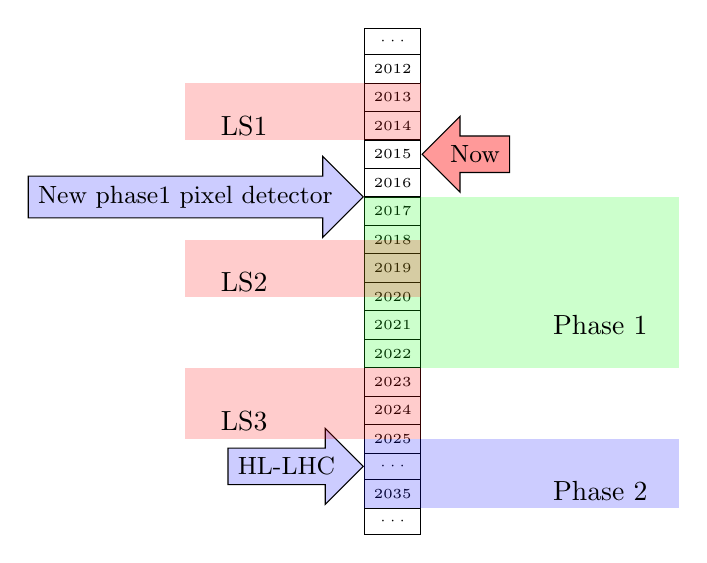
\begin{tikzpicture}
      %timeline
      \node [name=timeline, rectangle split, rectangle split parts=18, draw, anchor=center, font=\tiny] at (0,0) {
        $\cdots$\nodepart{two}2012\nodepart{three}2013\nodepart{four}2014\nodepart{five}2015\nodepart{six}2016\nodepart{seven}2017\nodepart{eight}2018\nodepart{nine}2019\nodepart{ten}2020\nodepart{eleven}2021\nodepart{twelve}2022\nodepart{thirteen}2023\nodepart{fourteen}2024\nodepart{fifteen}2025\nodepart{sixteen}$\cdots$\nodepart{seventeen}2035\nodepart{eighteen}$\cdots$};

      %arrows
      \draw[shift=(timeline.five east)] plot coordinates{(0,0)}
      node[arrow1] {Now};

      \onslide<2-> {
        \draw[shift=(timeline.six split west)] plot coordinates{(0,0)}
        node[arrow2] {New phase1 pixel detector};
      }

      \onslide<3-> {
        \draw[shift=(timeline.sixteen west)] plot coordinates{(0,0)}
        node[arrow2] {HL-LHC};
      }

      %phase rectangles
      \onslide<2-> {
        \fill[green, fill opacity=0.2, draw opacity=1] (timeline.six split west) rectangle coordinate[near end] (p1rec) ($ (timeline.twelve split west) + (4,0) $);
        \node at (p1rec) {Phase 1};
      }

      \onslide<3-> {
        \fill[blue, fill opacity=0.2, draw opacity=1] (timeline.fifteen west) rectangle coordinate[near end] (p2rec) ($ (timeline.seventeen split west) + (4,0) $);
        \node at (p2rec) {Phase 2};
      }

      %ls rectangles
      \fill[red, fill opacity=0.2, draw opacity=1] (timeline.two split east) rectangle coordinate[near end] (ls1rec) ($ (timeline.four split east) + (-3,0) $);
      \node at (ls1rec) {LS1};

      \fill[red, fill opacity=0.2, draw opacity=1] (timeline.eight east) rectangle coordinate[near end] (ls2rec) ($ (timeline.ten east) + (-3,0) $);
      \node at (ls2rec) {LS2};

      \fill[red, fill opacity=0.2, draw opacity=1] (timeline.twelve split east) rectangle coordinate[near end] (ls3rec) ($ (timeline.fifteen east) + (-3,0) $);
      \node at (ls3rec) {LS3};
    \end{tikzpicture}
  \end{center}
\end{frame}

% \begin{frame}
%   \frametitle{Tracker substitution}
%   \begin{center}
%     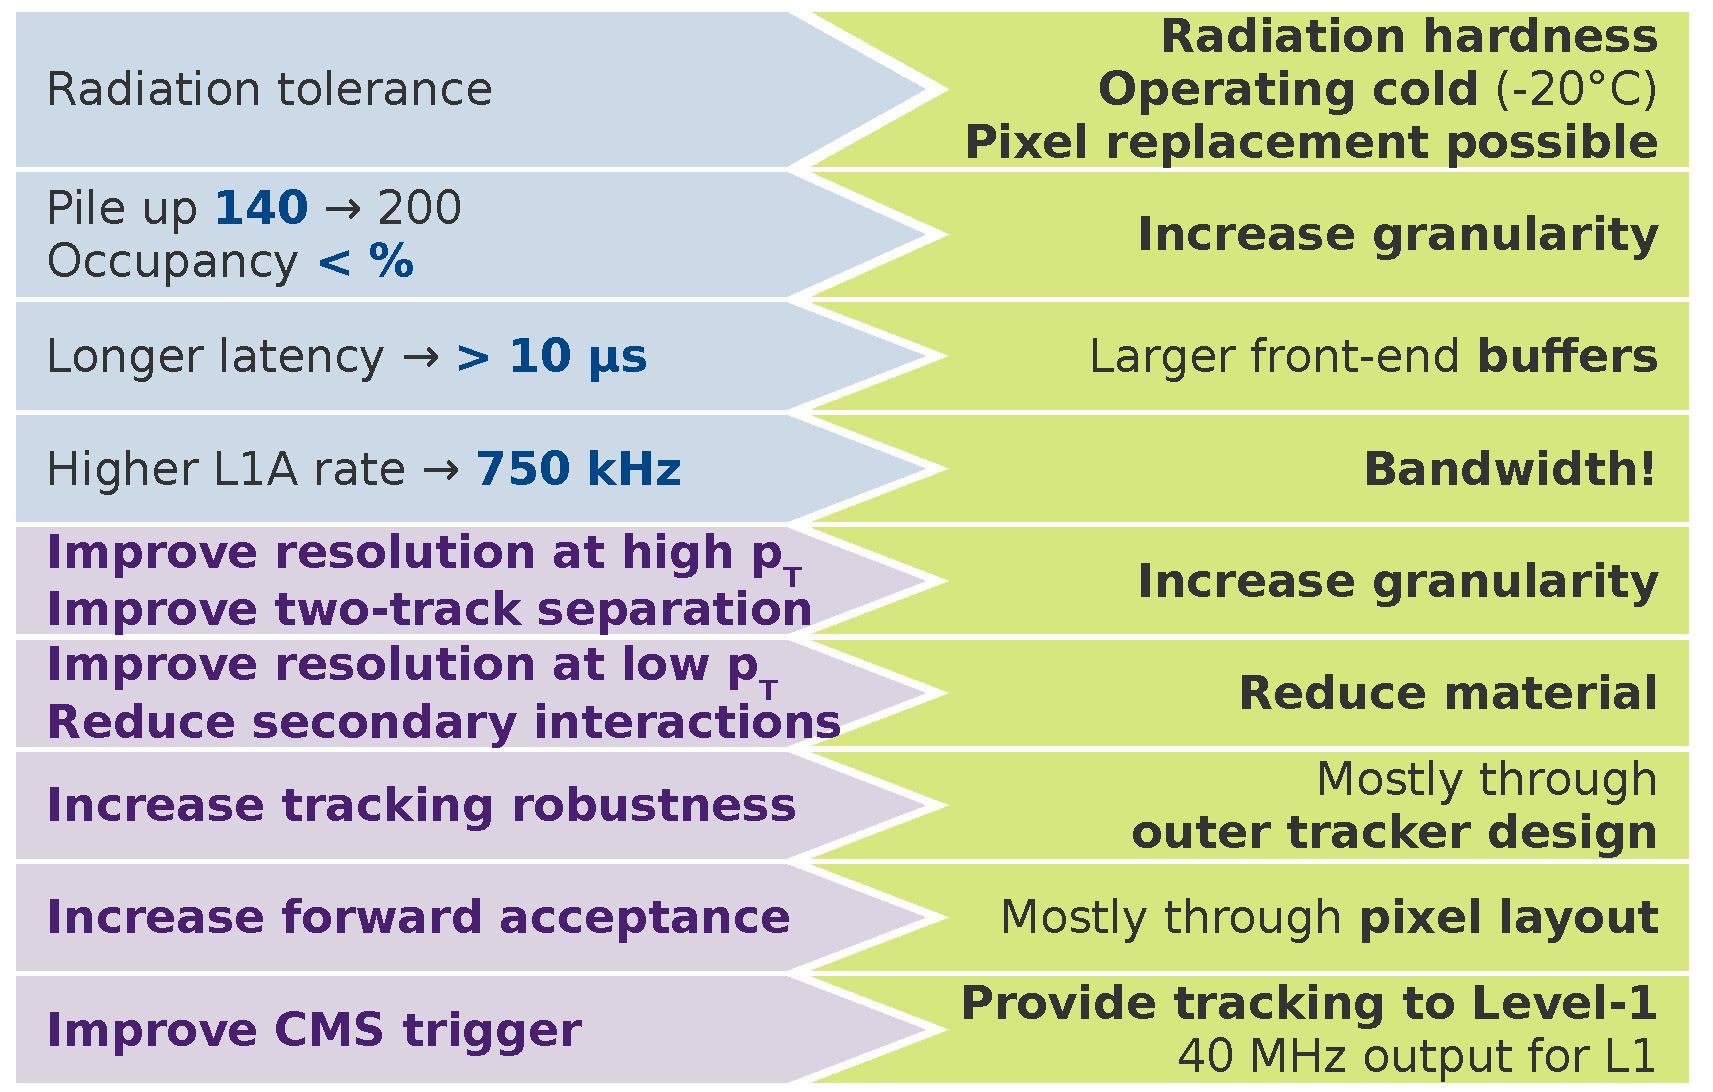
\includegraphics[width=\textwidth]{img/trackerSubs.pdf}
%   \end{center}
% \end{frame}

\begin{frame}[fragile]
  \frametitle{Trade off}
  \begin{center}
    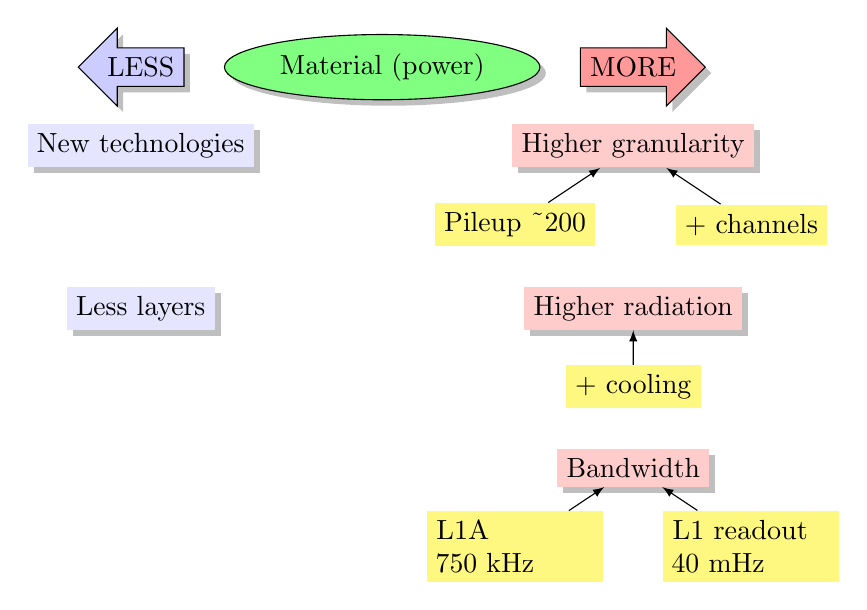
\begin{tikzpicture}[edge from parent/.style={draw,latex-}, level 1/.style={sibling distance=3cm}, level distance=1cm]
      %arrows
      \node[powmat] (powmatn) at (0,0) {Material (power)};
      \onslide<2-> { \node[arrowR] (mormat) at ($ (powmatn.east) + (0.5,0) $) {MORE}; }
      \onslide<5-> { \node[arrowL] (lessmat) at ($ (powmatn.west) - (0.5,0) $) {LESS}; }

      \pause
      %under more
      \node[underboxr, below of=mormat] (higran) {Higher granularity}
      child { node[underunderbox] {Pileup \textasciitilde 200}}
      child { node[underunderbox] {+ channels}};
      \pause
      \node[underboxr, below= 1.5cm of higran] (hirad) {Higher radiation}
%      child { node {+ consumption}}
      child { node[underunderbox] {+ cooling}};
      \pause
      \node[underboxr, below= 1.5cm of hirad] (band) {Bandwidth}
      child { node[underunderbox, text width=2cm] {L1A 750~kHz}}
      child { node[underunderbox, text width=2cm] {L1 readout 40~mHz}};

      \pause
      %under less
      \node[underboxl, below of=lessmat] (newtec) {New technologies};
%     child { node {Can affect performance} edge from parent[-latex]};
      \pause
      \node[underboxl, below= 1.5cm of newtec] (lesslay) {Less layers};
    \end{tikzpicture}
  \end{center}
\end{frame}

\begin{frame}
  \frametitle{Tracker layout}
  \begin{center}
    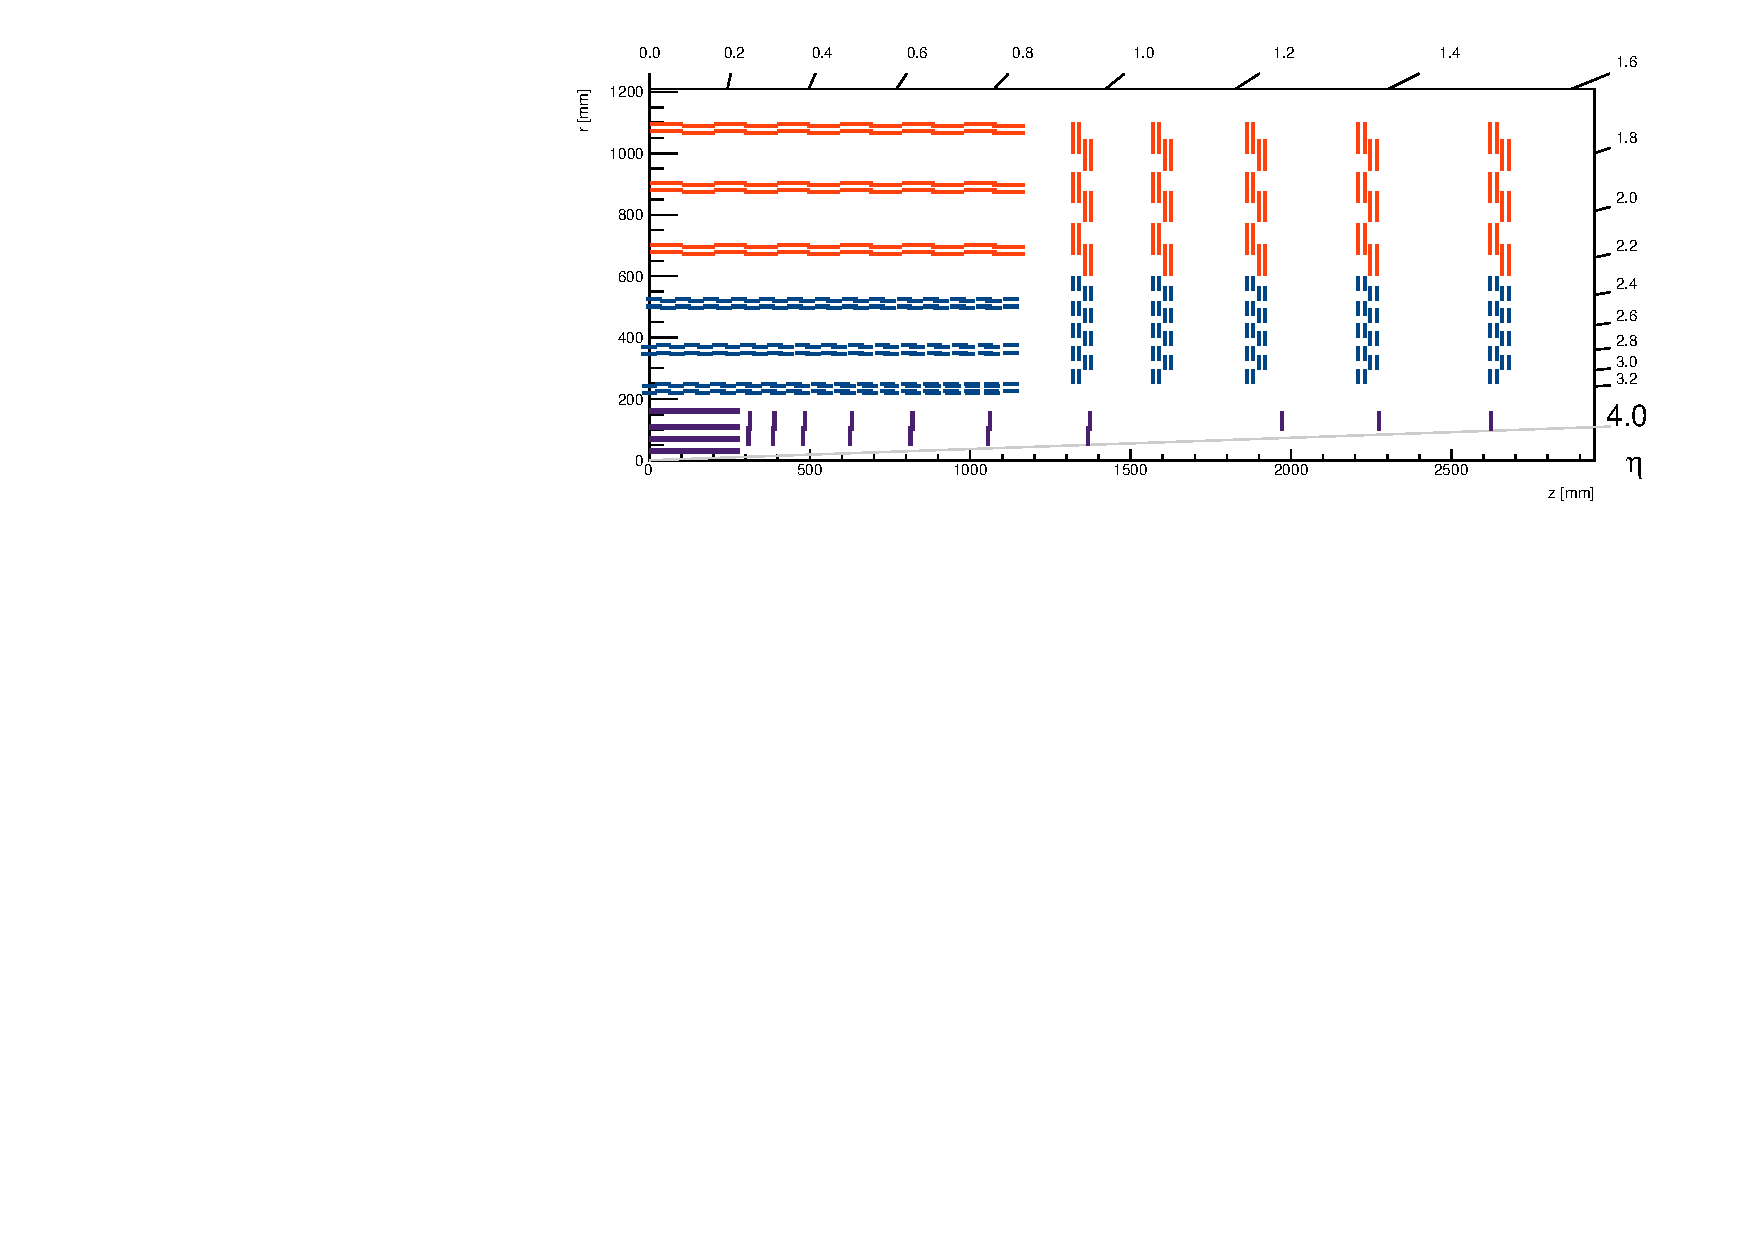
\includegraphics[width=\textwidth]{img/fullLayout.pdf}
  \end{center}
\tikz[baseline, overlay]\node<2-> [evidenziaRett, minimum width = 3.8cm, minimum height = 1.3cm] at (3.15cm,4.1cm) {TB2S};
\tikz[baseline, overlay]\node<3-> [evidenziaRett, minimum width = 3.7cm, minimum height = 1cm] at (3cm,2.6cm) {TBPS};
\tikz[baseline, overlay]\node<4-> [evidenziaRett, minimum width = 4.55cm, minimum height = 2.75cm] at (7.5cm,3.5cm) {TEDD};
\tikz[baseline, overlay]\node<5-> [evidenziaRett, minimum width = 9cm, minimum height = 0.5cm] at (5.3cm,1.6cm) {PIXEL};
\end{frame}

\begin{frame}
  \frametitle{Endcaps mechanics (2S \& PS)}
  \begin{center}
    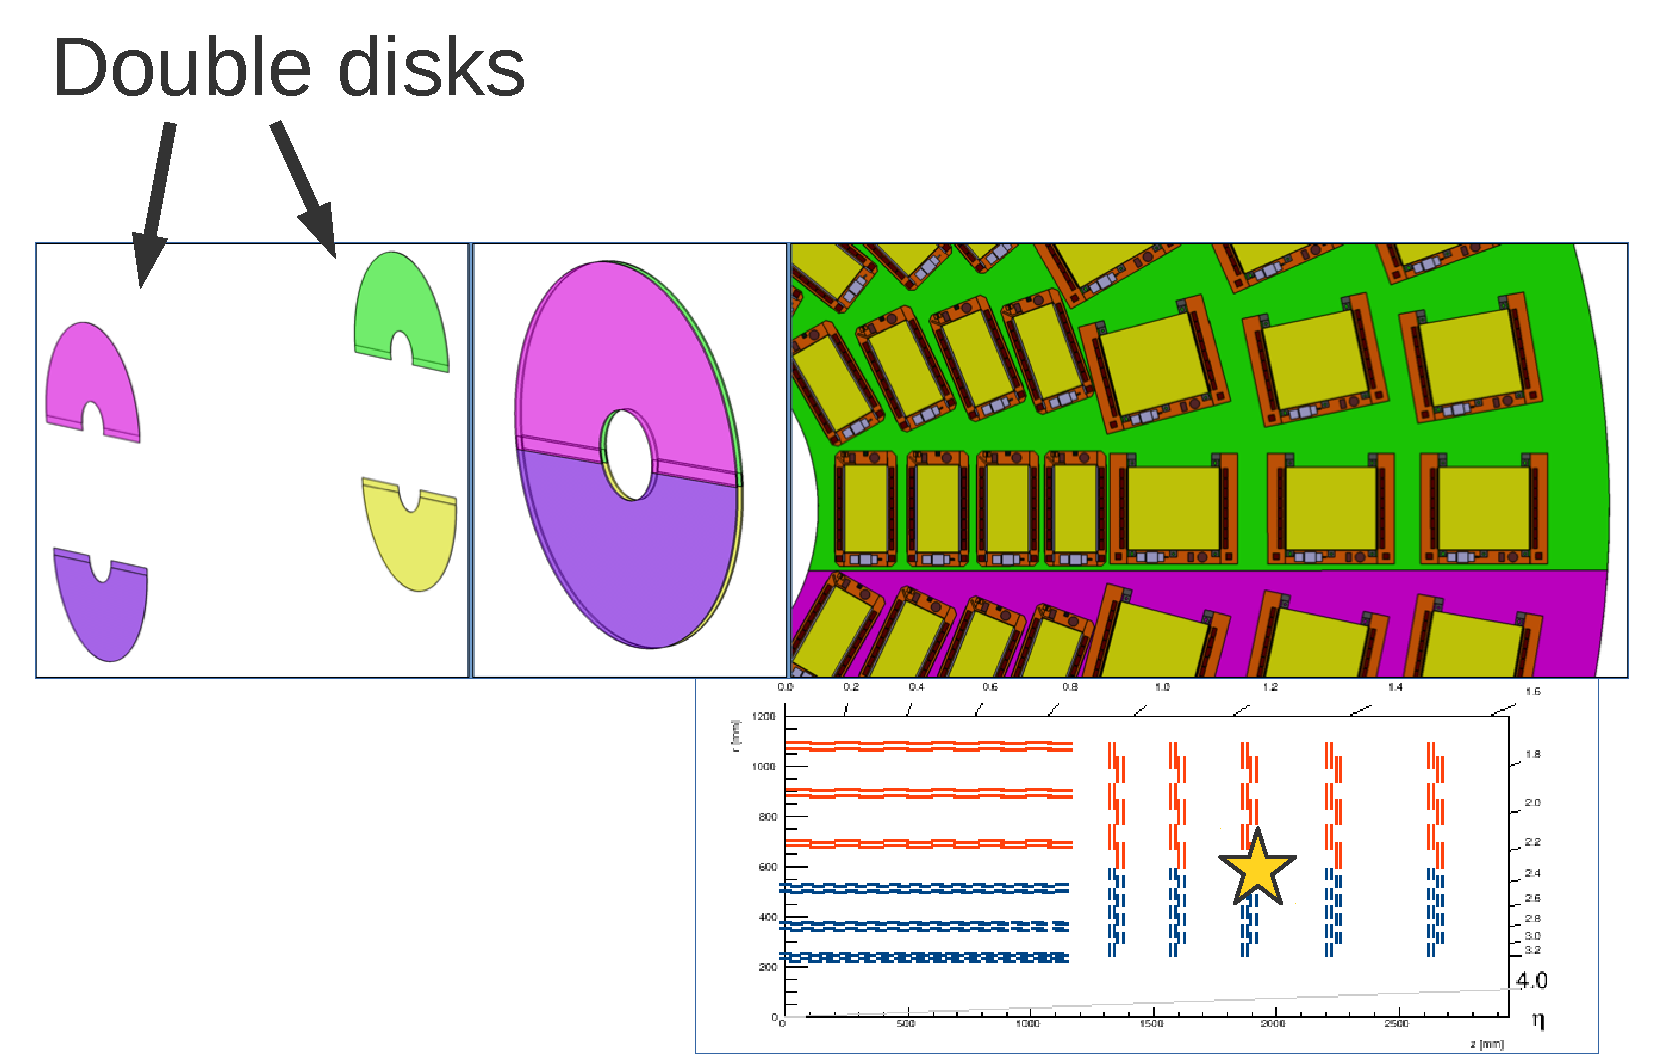
\includegraphics[width=\textwidth]{img/mechanics1.pdf}
  \end{center}
\end{frame}

\begin{frame}
  \frametitle{Barrel mechanics (2S)}
  \begin{center}
    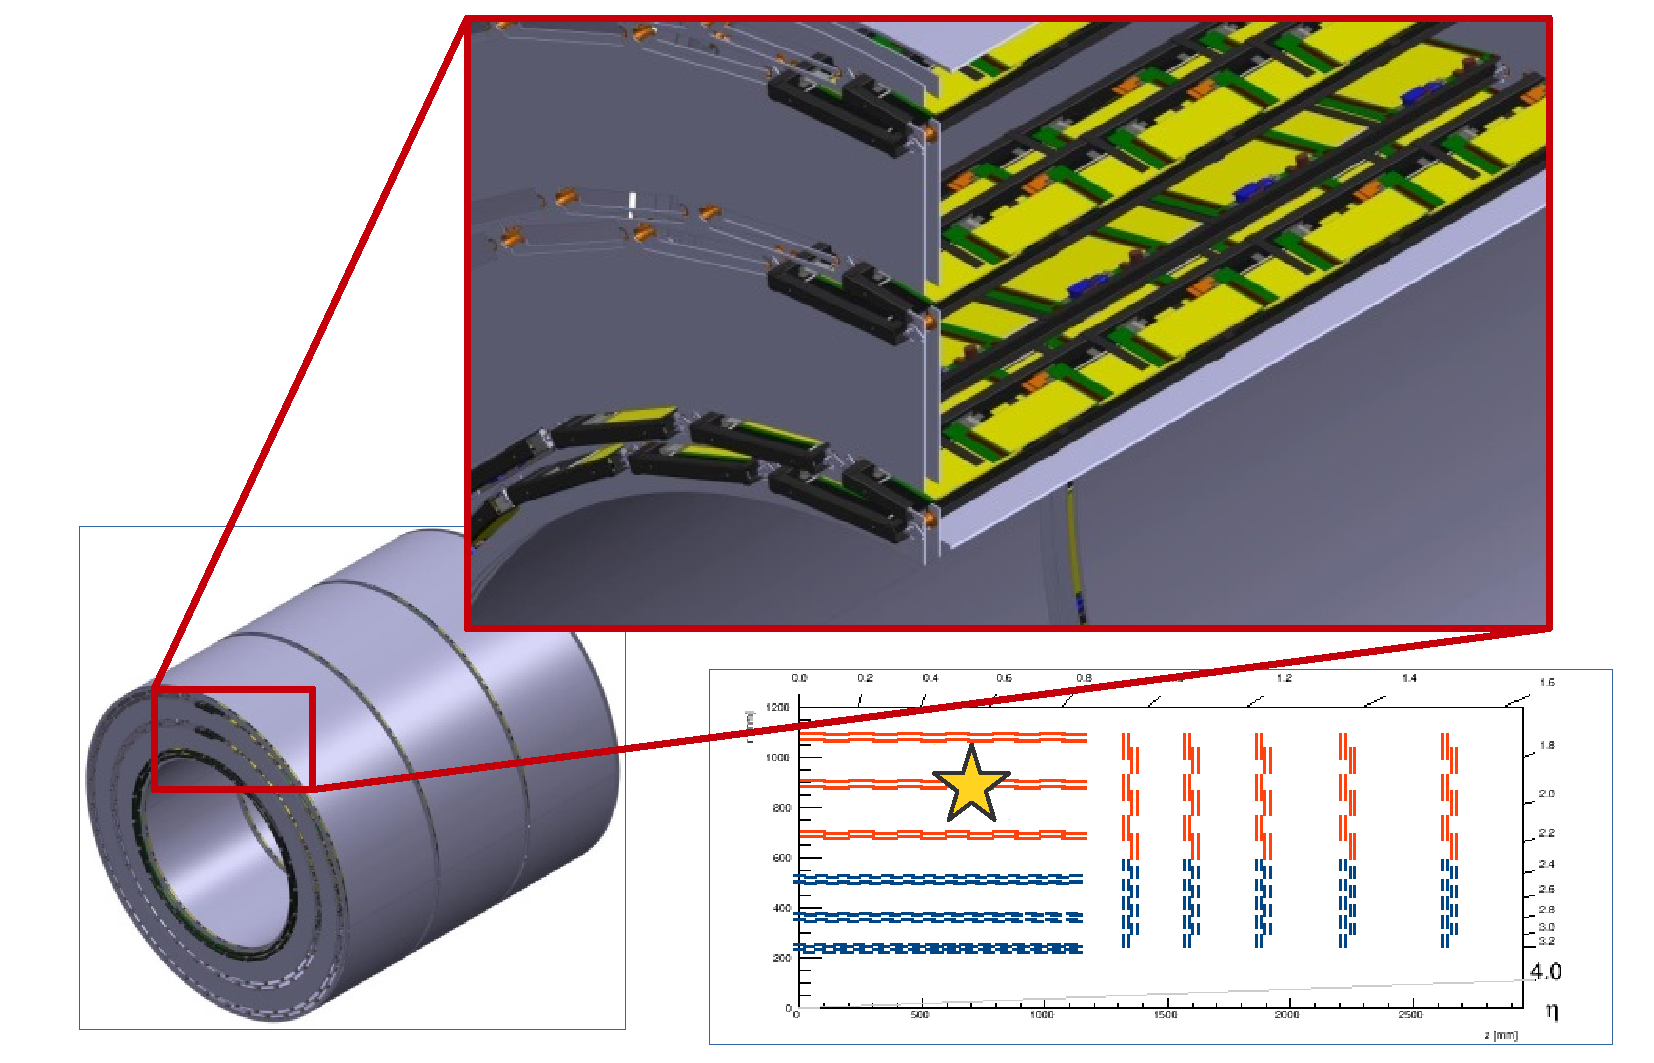
\includegraphics[width=\textwidth]{img/mechanics2.pdf}
  \end{center}
\end{frame}

\begin{frame}
  \frametitle{Barrel mechanics (PS)}
  \begin{center}
    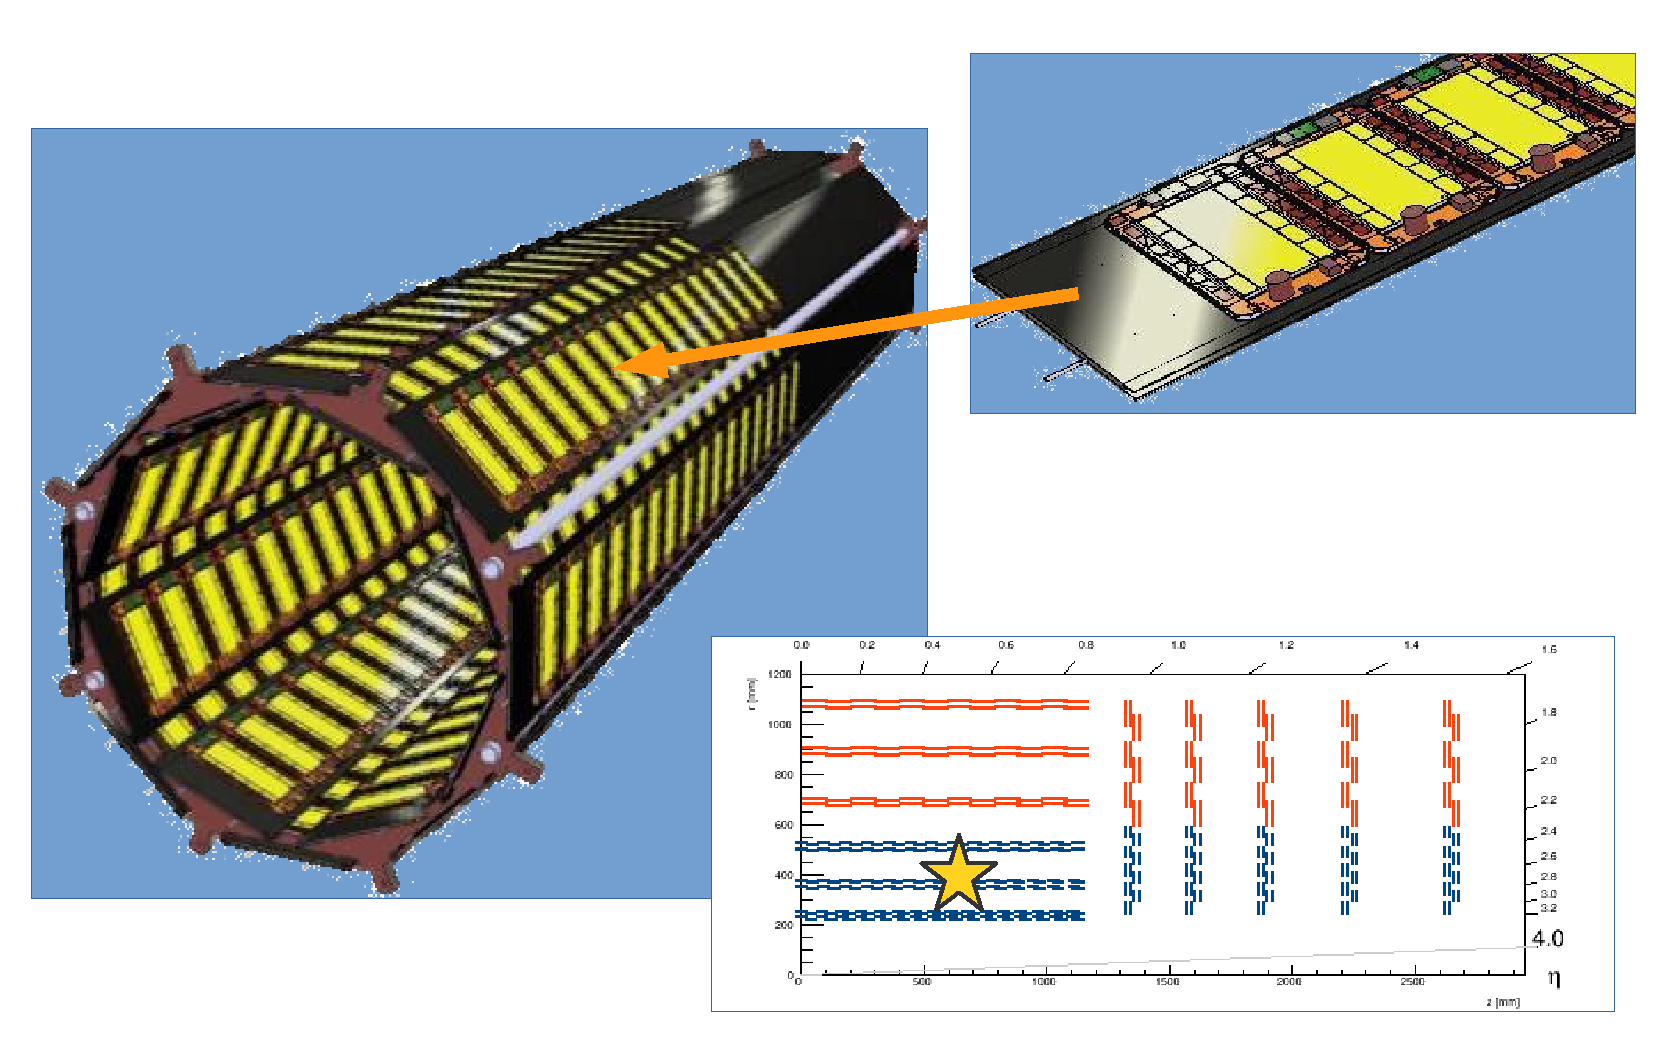
\includegraphics[width=\textwidth]{img/mechanics3.pdf}
  \end{center}
\end{frame}

\begin{frame}
  \frametitle{Barrel mechanics (PS alternative)}
  \begin{center}
    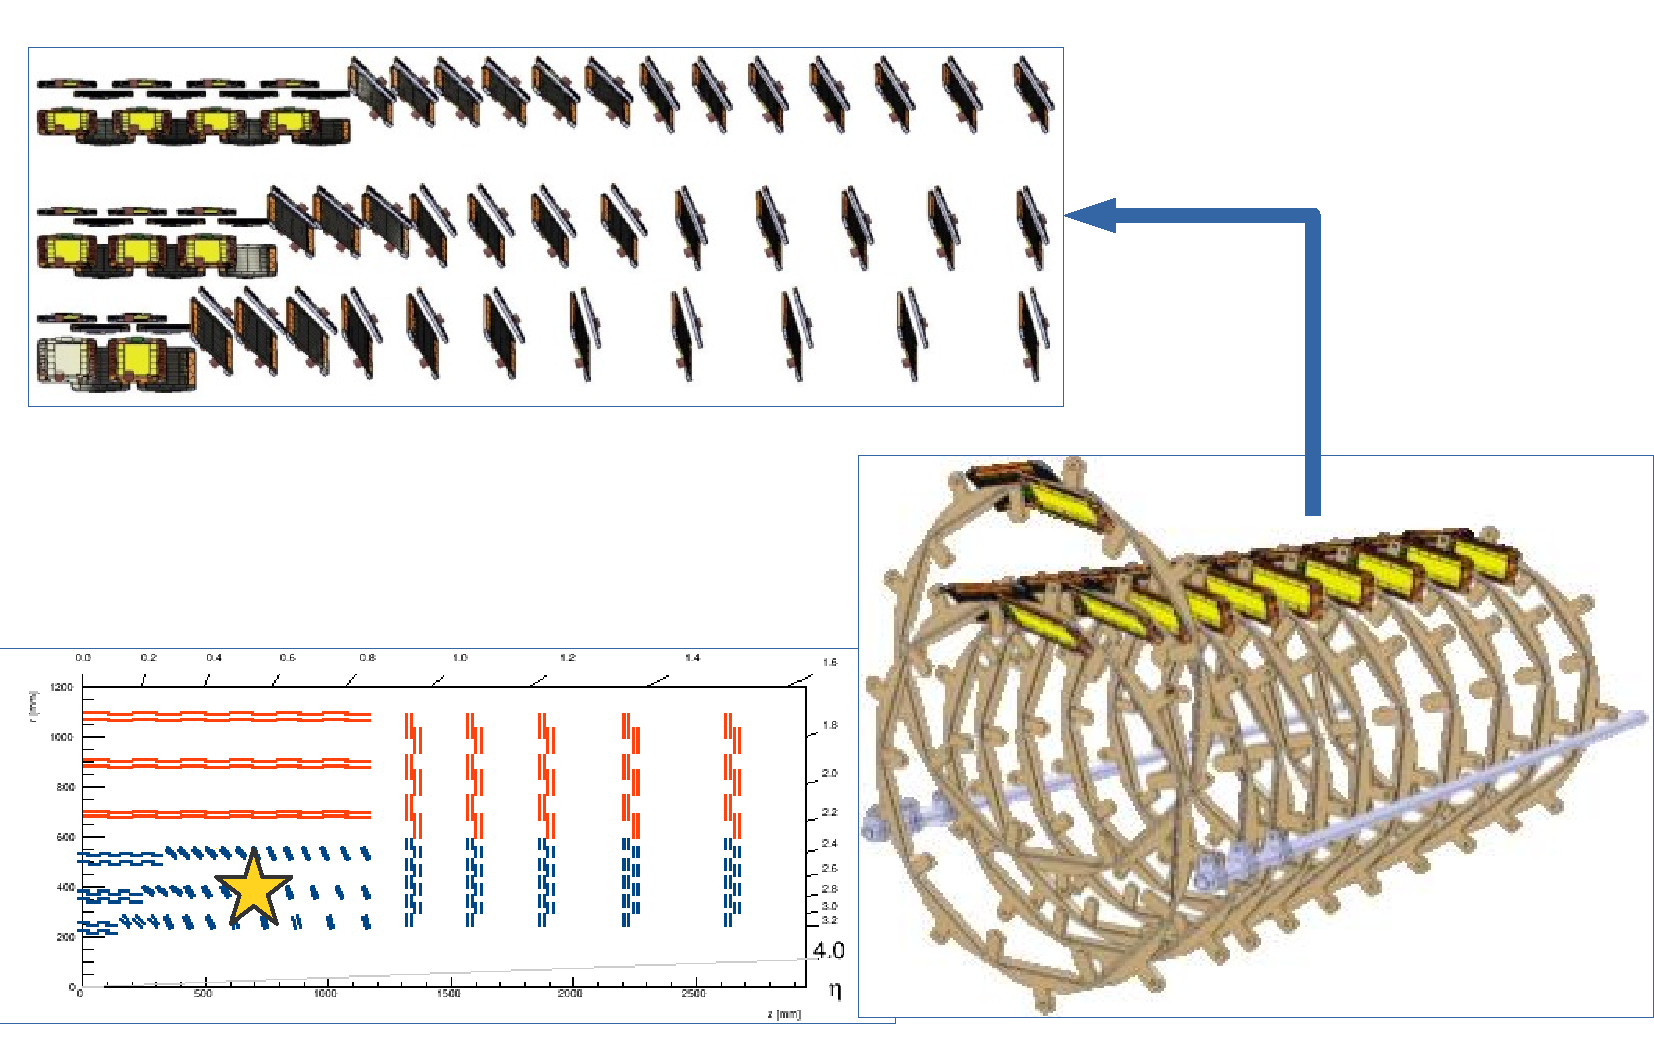
\includegraphics[width=\textwidth]{img/mechanics4.pdf}
  \end{center}
\end{frame}

\begin{frame}
  \frametitle{Target}
  \begin{itemize}
  \item Evaluate \alert{material} amount (aim to a lighter tracker with respect to the current one)
    \pause
  \item Evaluate tracking \alert{performance}
  \end{itemize}
\end{frame}

\begin{frame}
  \frametitle{Status}
  \begin{itemize}
  \item We know how to build \alert{modules} for outer
  \item<2-> not yet for pixel
  \item<3-> we have a fairly \alert{stable} design for the \alert{TB2S} and \alert{TEDD}
  \item<4-> we have two \alert{competing} concepts for the \alert{TBPS}
  \item<5-> the \alert{pixel} detector design is much less detailed 
  \end{itemize}
  \begin{center}
    \visible<3-> {
      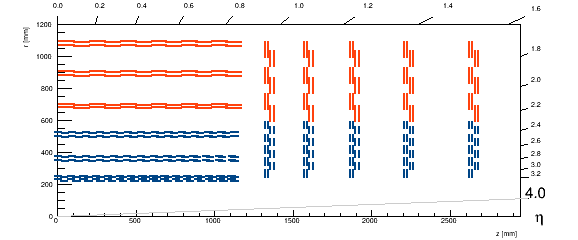
\includegraphics[width=\textwidth/2]{img/layoutNorm.png}
    }
  \end{center}
  \begin{center}
    \visible<4-> {
      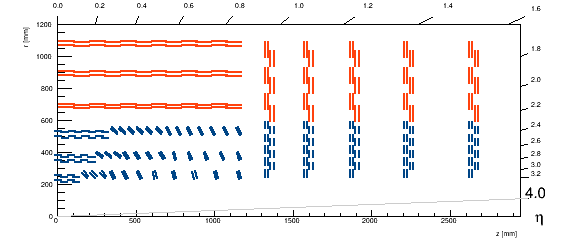
\includegraphics[width=\textwidth/2]{img/layoutTilt.png}
    }
  \end{center}

  \tikz[baseline, overlay]\node<3> [evidenziaRett, minimum width = 2cm, minimum height = 1cm] at (4.6cm,5.2cm) {};
  \tikz[baseline, overlay]\node<3> [evidenziaRett, minimum width = 2.2cm, minimum height = 1.5cm] at (6.8cm,4.9cm) {};

  \tikz[baseline, overlay]\node<4> [evidenziaRett, minimum width = 2cm, minimum height = 0.7cm] at (4.6cm,4.77cm) {};
  \tikz[baseline, overlay]\node<4> [evidenziaRett, minimum width = 2cm, minimum height = 0.7cm] at (4.5cm,2.1cm) {};

  % \begin{center}
  %   \begin{tikzpicture}
  %     \onslide<2>{
  %       \node[node1, text width=3cm] (innoTilt) at (0,0) {Tilted barrel reduce precision};
  %       \node[node1, below right=1cm and 0.5cm of innoTilt] (innoTrad) {Trade off};
  %       \node[node2, below right=1cm and 0.5cm of innoTrad, text width=3cm] (innoInst) {Instrument for analysing material distribution and performance};
        
  %       \path[bend right, arrow] (innoTilt) edge (innoTrad);
  %       \path[bend right, arrow] (innoTrad) edge (innoInst);
  %     }
  %   \end{tikzpicture}
  % \end{center}
\end{frame}

\begin{frame}
  \begin{enumerate}
  \item in order to \alert{study} the \alert{pixel} detector a more \alert{detailed} radiation
    \alert{map} of the inner region was needed, along with a coarser, but
    wider radiation map for the outer tracker
    \pause
  \item the \alert{tilted} barrel option offers an attractive \alert{reduction} of
    number of \alert{modules} needed (less material and lower cost), at the
    potential expense of \alert{z0 resolution} in the trigger readout
    (comparative study needed)
    \pause
  \item \alert{material} from \alert{pixel} detector \alert{effect} on tracking resolution is to be quantified 
  \end{enumerate}
  \pause
  \begin{block}{Solution}
    \begin{description}
    \item[1 $\rightarrow$] more \alert{flexible} input of \alert{FLUKA} radiation maps into tkLayout
    \item[2,3 $\rightarrow$] completely \alert{rework} the \alert{model} of \alert{material} (see later)
    \end{description}
  \end{block}
\end{frame}

\begin{frame}
  \frametitle{TkLayout main features}
  \begin{itemize}
  \item predict \alert{material} distribution and effects
    \pause
  \item predict \alert{resolution}
    \pause
%  \item<3-> generate \alert{modules} definition for mechanical
  \item generate \alert{CMSSW} input files for simulation (XML with geometry)
    \pause
  \item evaluate \alert{tilted} barrel and \alert{pixel}
  \end{itemize}
  \pause
  \begin{block}{Using}
    \begin{itemize}
    \item error \alert{propagation}
    \item \alert{not} use simulations
      \begin{itemize}
      \item[$\rightarrow$] \alert{fast} analysis
      \end{itemize}
    \end{itemize}
  \end{block}
\end{frame}

\begin{frame}
  \frametitle{Importance of material}
  \begin{itemize}
  \item material is important for determine the
    \alert{resolution} of phase2 tracker
  \end{itemize}
  \begin{center}
%    \visible<2>{
      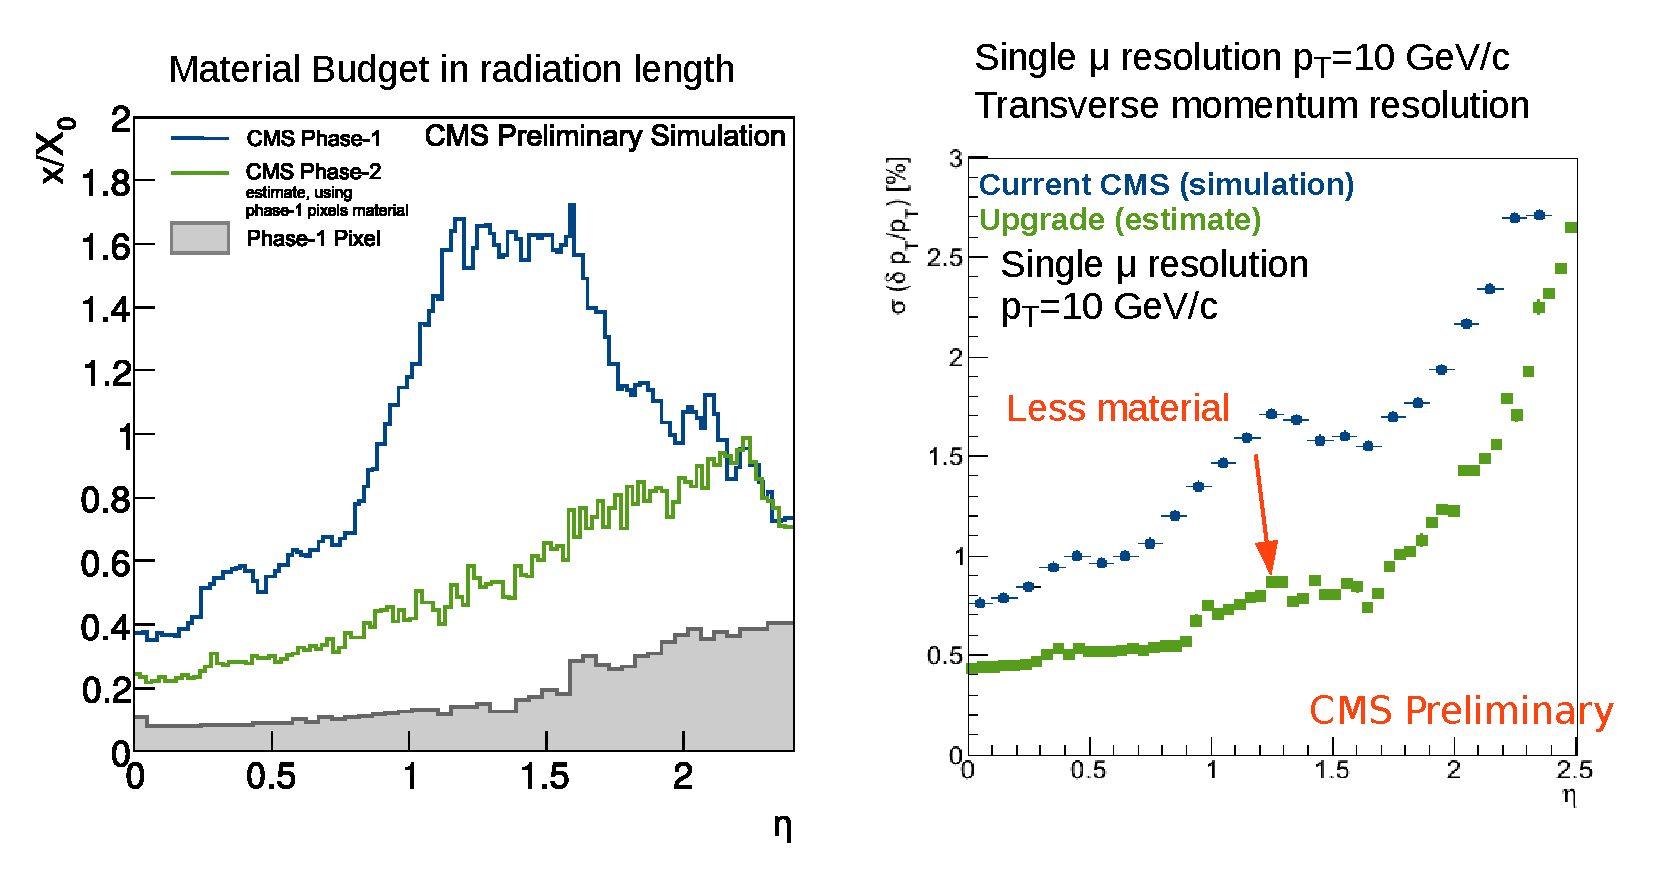
\includegraphics[width=\textwidth]{img/trackMatRes.pdf}
%    }
    % \includegraphics<3>[width=\textwidth]{img/trackRes.pdf}
    % \visible<4>{
    %   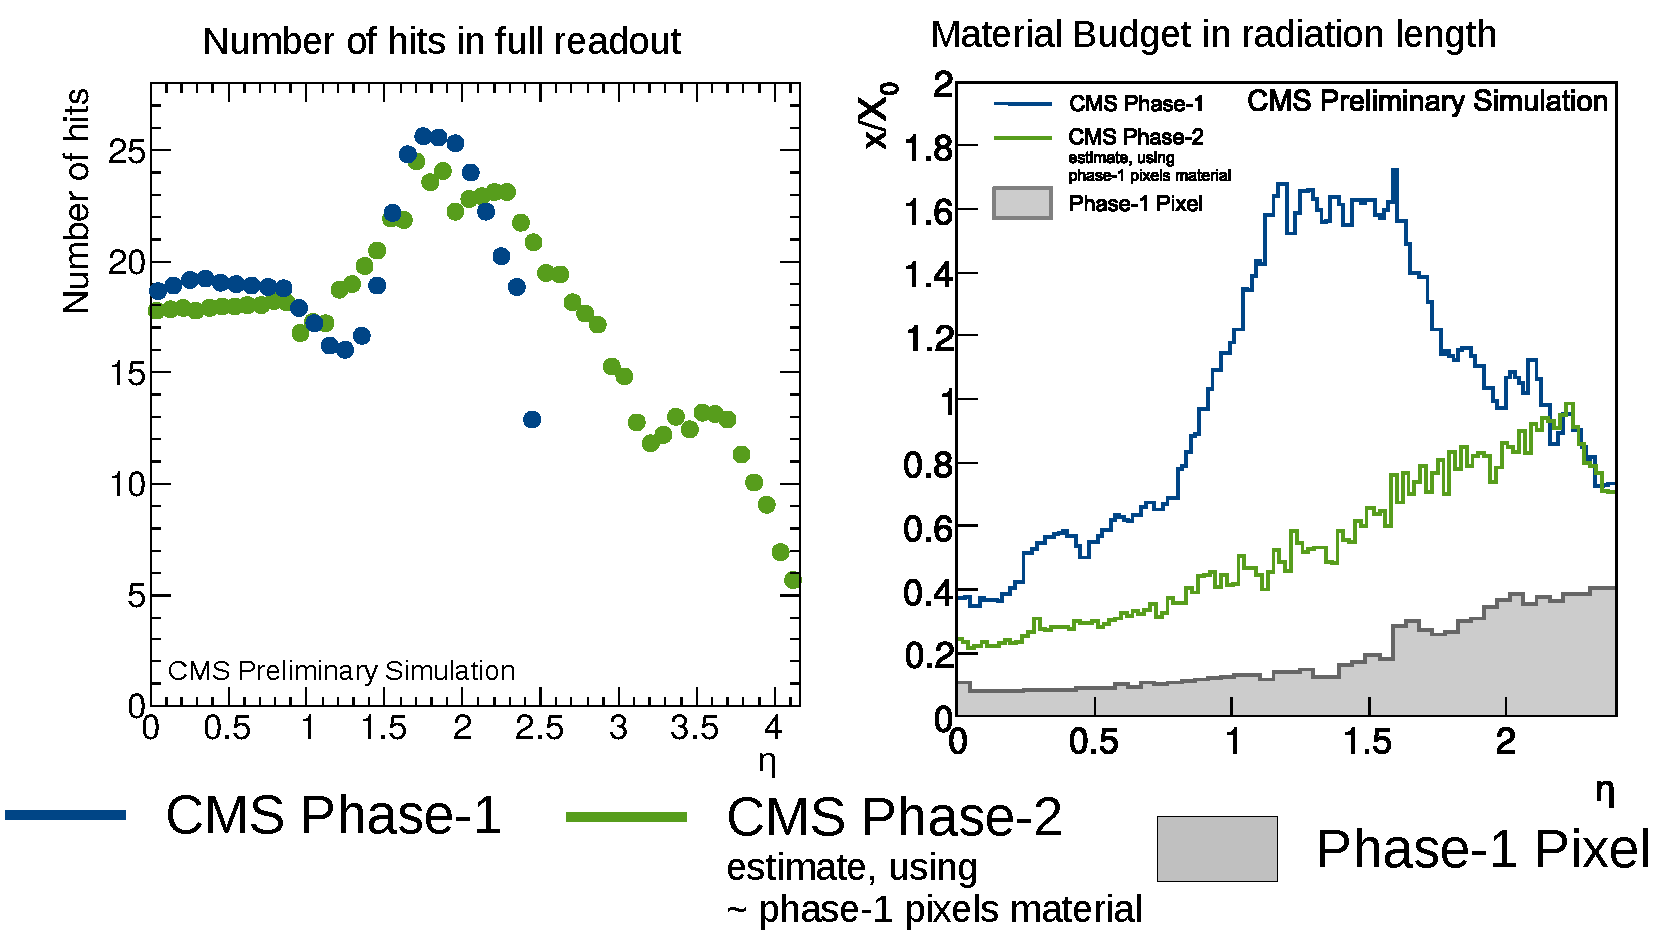
\includegraphics[width=\textwidth]{img/trackMat.pdf}
    % }
  \end{center}
\end{frame}

% \begin{frame}
%   \frametitle{Phase 2}
%   \begin{itemize}
%   \item \alert{outer tracker} at advanced study phase
%     \begin{itemize}
%     \item \alert{TB2S} consolidate
%     \item \alert{TBPS} still different options
%       \begin{itemize}
%       \item \alert{flat}
%       \item \alert{tilted}
%       \end{itemize}
%     \end{itemize}
%   \item \alert{pixel} not well designed model
%     \begin{itemize}
%     \item power?
%     \item laser?
%     \end{itemize}
%   \end{itemize}
% \end{frame}

% \begin{frame}
%   \frametitle{\tkl for phase 2}
%   \begin{itemize}
%   \item \alert{monitor} material budget
%   \item \alert{design} for pixel
%   \end{itemize}
% \end{frame}

\begin{frame}[fragile]
%  \frametitle{Example configuration}
  \tiny
  \begin{block}{\pat{.../geometries/Baseline2015}}
\begin{verbatim}
Tracker Outer {
    @include Baseline2015_SupportsTracker.cfg

    // Layout construction parameters
    zError 70
    bigDelta 12
    zOverlap 1
    phiOverlap 1
    etaCut 10
    barrelRotation 1.57079632679
    smallParity 1

    trackingTags trigger,tracker

    Barrel TBPS {
      @include Baseline2015_SupportsBarrelTBPS.cfg
      Layer 1   { smallDelta 3.65 }
      Layer 2,3 { smallDelta 3.15 }
      numLayers 3
      maxZ 1150
      startZMode modulecenter
      innerRadius 230
      outerRadius 508 // 509 or 540
      width 96
      length 46.26
      physicalLength 71
      phiSegments 2
    }
...
\end{verbatim}
  \end{block}
\end{frame}


%\foreach \n in {1,3,4}{
\begin{frame}
\frametitle{Geometry}
  \begin{center}
    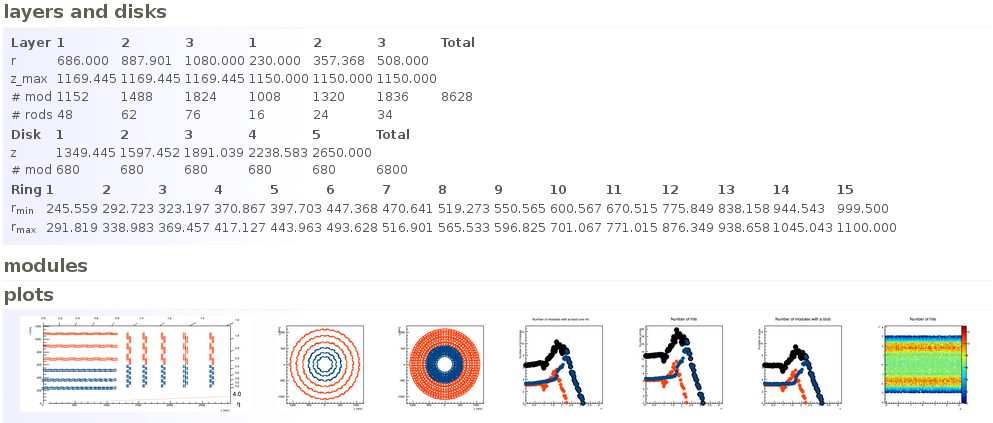
\includegraphics[width=\textwidth]{img/screenshot1.png}
  \end{center}
\end{frame}
%}

\begin{frame}
\frametitle{Material distribution 1D}
  \begin{center}
    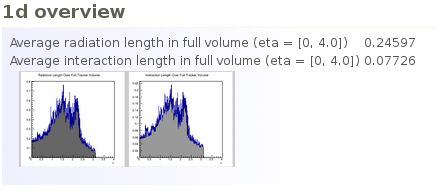
\includegraphics[width=\textwidth-4cm]{img/screenshot3.png}
  \end{center}
  \begin{center}
    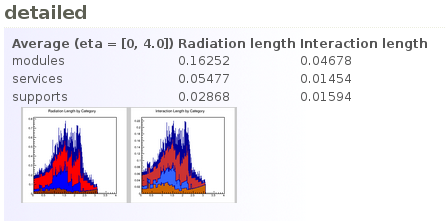
\includegraphics[width=\textwidth-4cm]{img/screenshot4.png}
  \end{center}
\end{frame}

\begin{frame}
  \begin{center}
    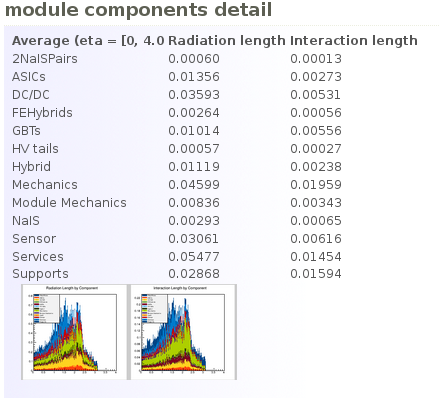
\includegraphics[width=\textwidth-2.5cm]{img/screenshot5.png}
  \end{center}
\end{frame}

\begin{frame}
\frametitle{Material distribution 2D}
  \begin{center}
    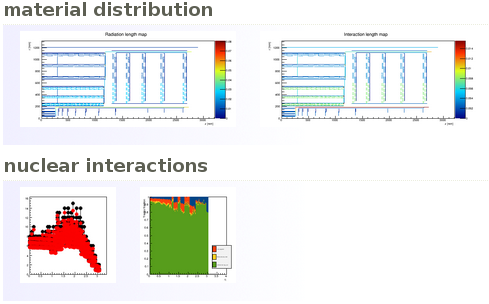
\includegraphics[width=\textwidth]{img/screenshot6.png}
  \end{center}
\end{frame}


% \foreach \n in {1,...,2}{
%   \begin{frame}
%     \begin{center}
%       \includegraphics[width=\textwidth]{img/screenshotPdf\n.pdf}
%     \end{center}
%   \end{frame}
% }

\begin{frame}
  \frametitle{My contribution to the project}
  \begin{itemize}
  \item \alert{radiation maps}
    \pause
    \begin{itemize}
    \item \alert{multiple} maps possible
    \item more \alert{detail}
      \pause
    \item useful for \alert{pixel} study
    \end{itemize}
    \pause
  \item new \alert{material} model
    \pause
    \begin{itemize}
    \item configuration \alert{files} definition
    \item internal \alert{representation}
    \item routing \alert{algorithm}
      \pause
    \item useful for \alert{tilted} barrel and \alert{pixel} study
    \end{itemize}
    \pause
  \item small \alert{bug-fix} and improvements
  \end{itemize}
\end{frame}

\begin{frame}
  \frametitle{Irradiation maps}
  \begin{itemize}
  \item \alert{Features} in irradiation maps
    \pause
    \begin{itemize}
    \item Presence of an \alert{header} with map properties
      \pause
    \item Presence of \alert{multiple maps} with different resolutions
      and size
    \end{itemize}
    \pause
  \item Values are \alert{read} and interpreted directly from the header
    \pause
  \item created a \alert{manager} that \alert{contains} any number of maps and use the one
    with the better resolution for every module
  \end{itemize}
  \visible<6> {
    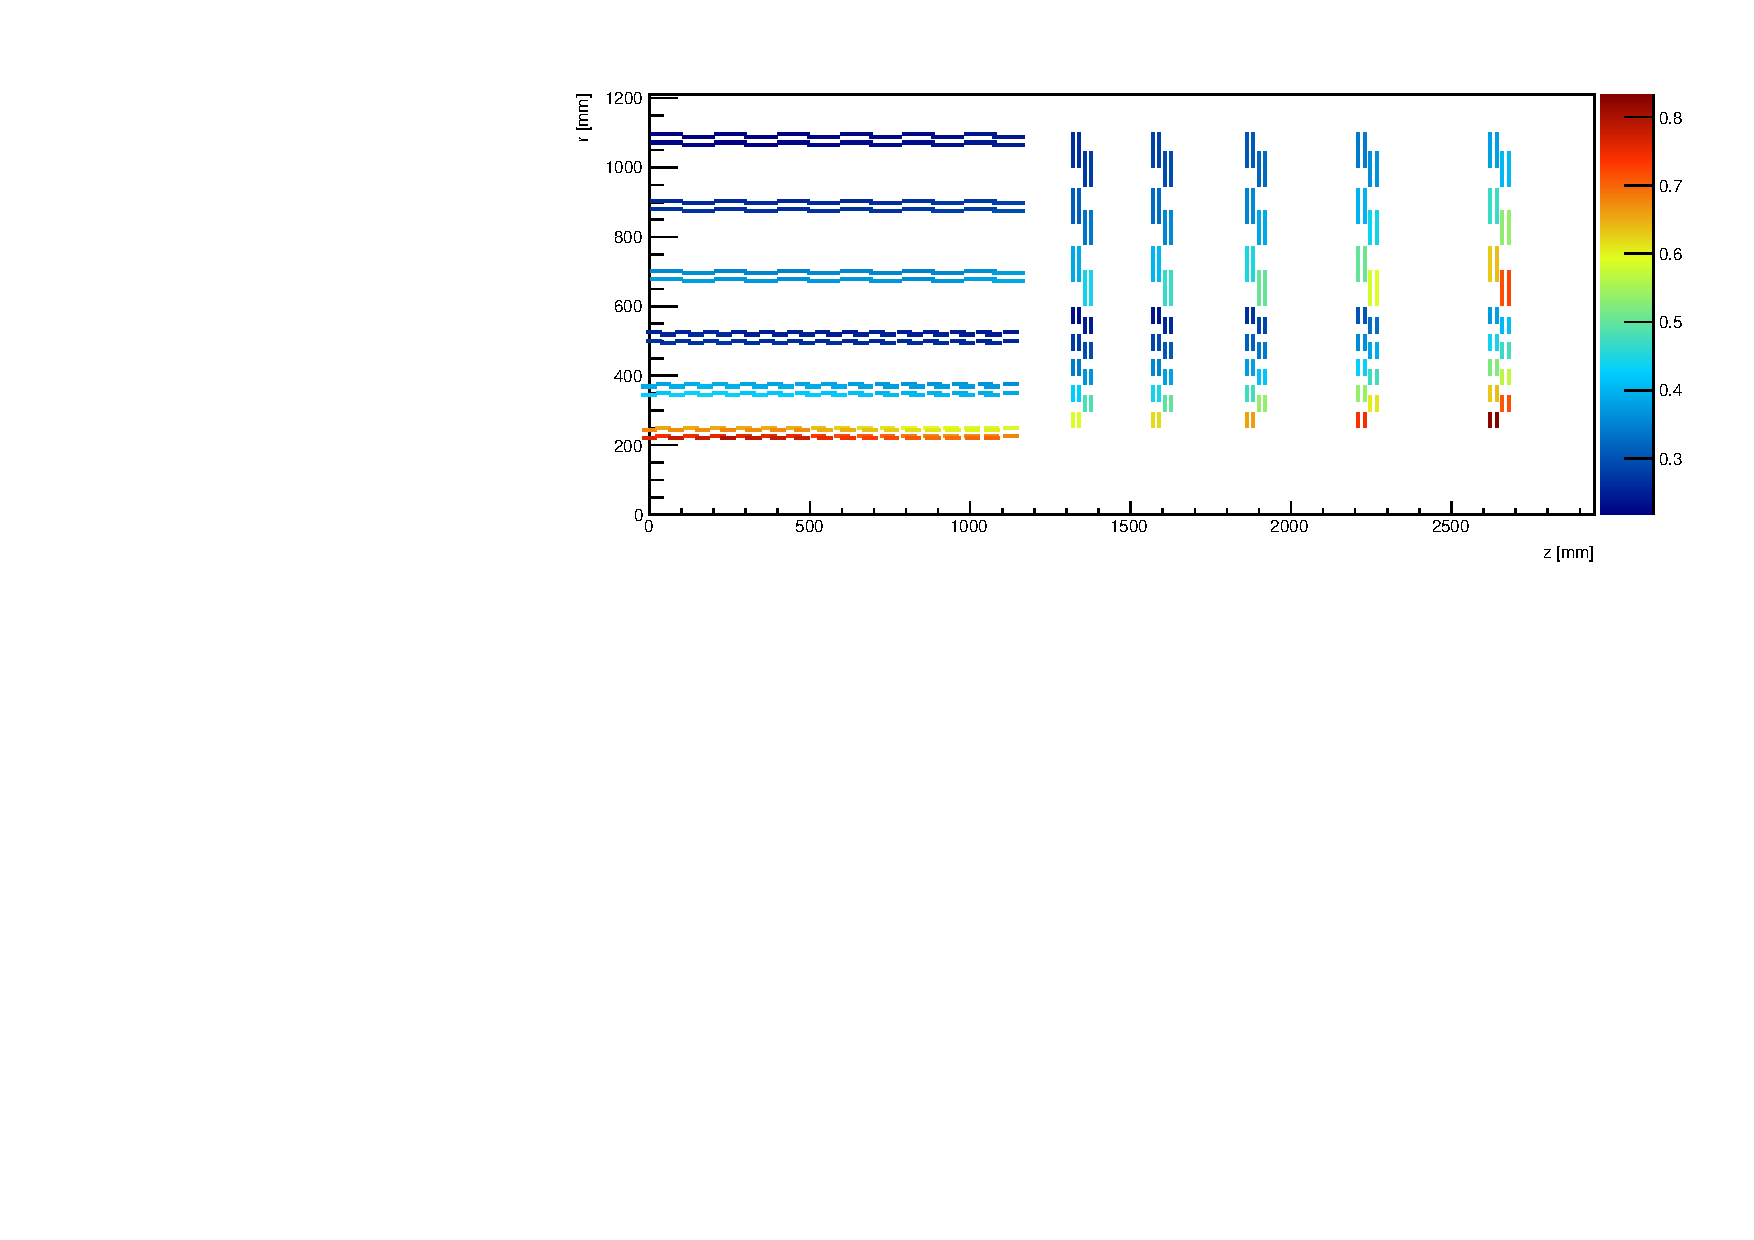
\includegraphics[width=\textwidth-0.5cm]{img/irradiation.pdf}
  }
\end{frame}


\begin{frame}{Old material model}
  \begin{center}
    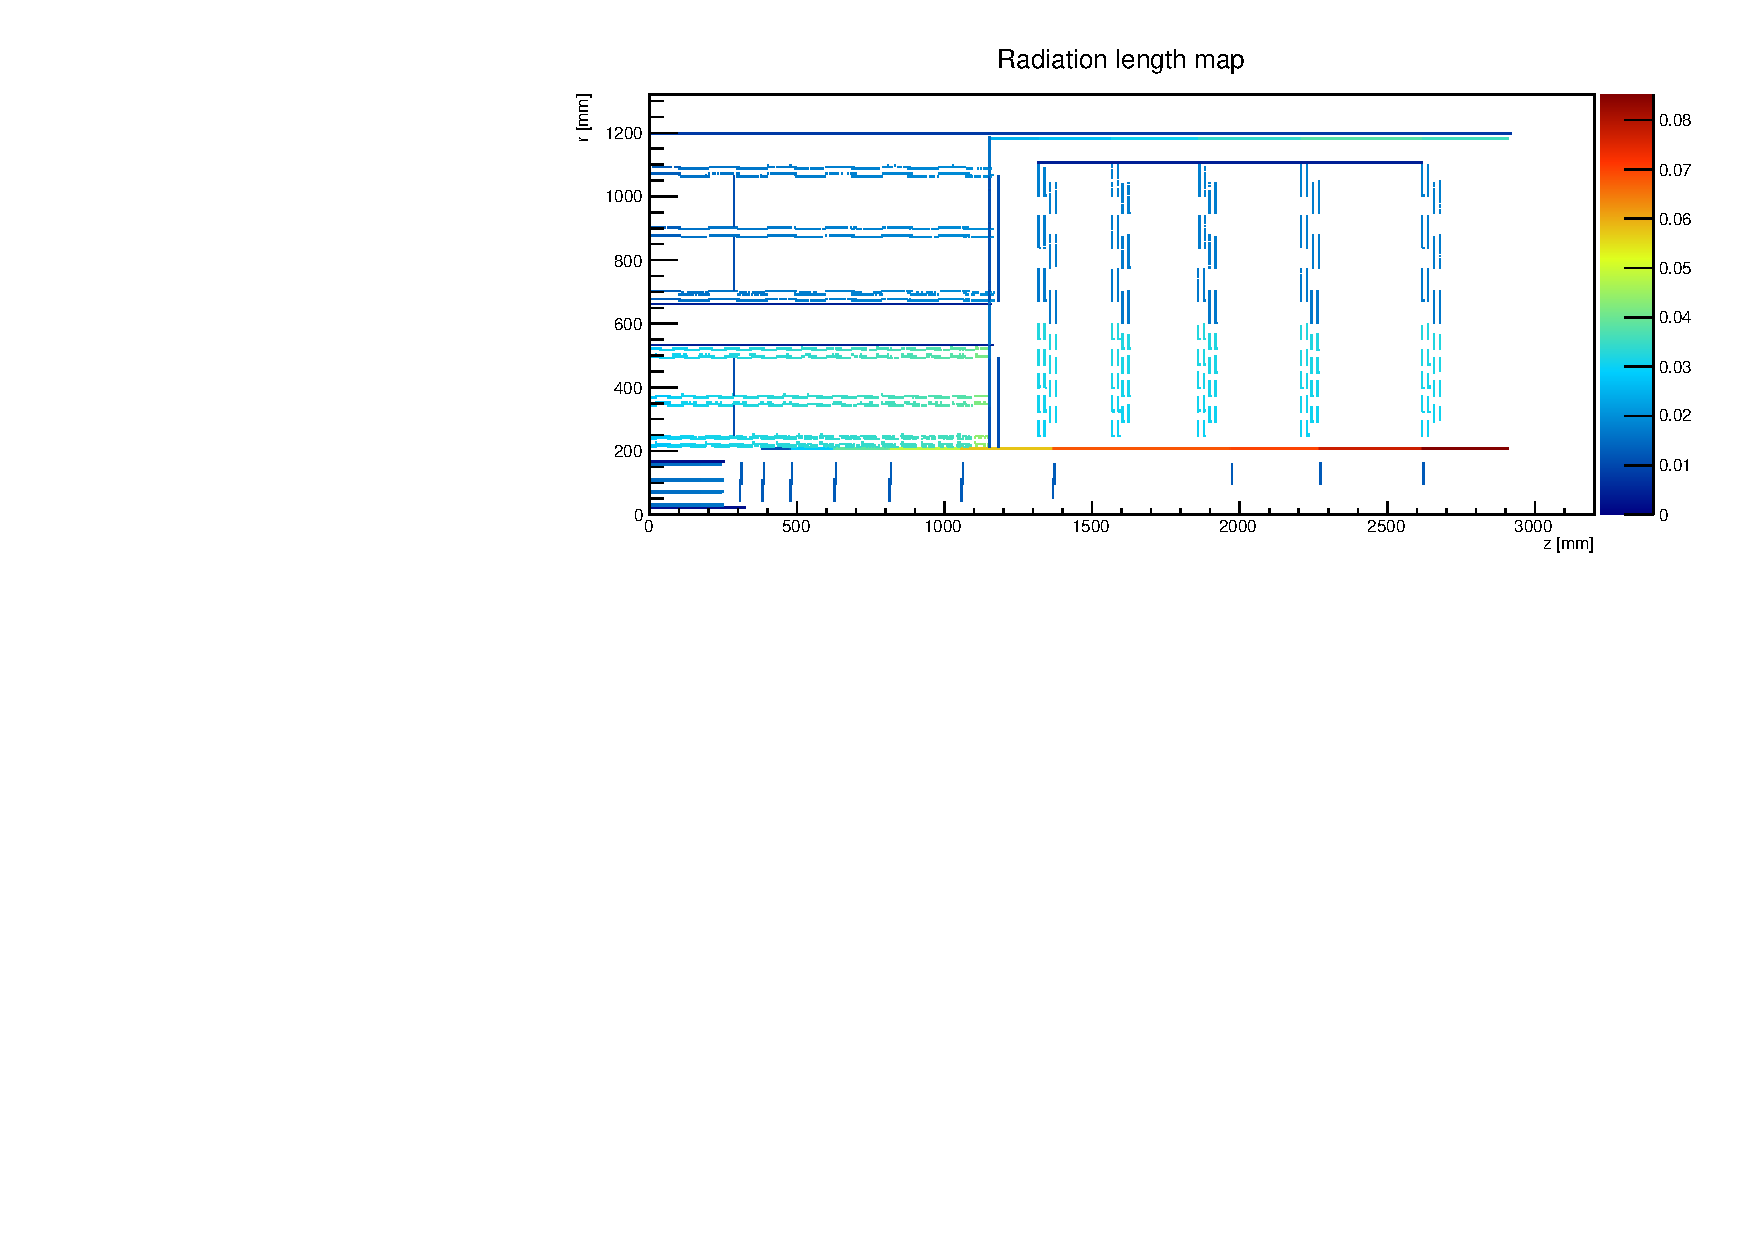
\includegraphics[width=\textwidth]{img/oldModel.pdf}
  \end{center}
  \begin{itemize}
  \item Cables material distributed \alert{inside} modules volumes
    \pause
  \item Possible to model \alert{cooling pipe} along rods, \alert{manifold} in the flange and bigger cooling pipe out of the barrel
  \end{itemize}
\end{frame}

\begin{frame}{New material model}
  \begin{center}
    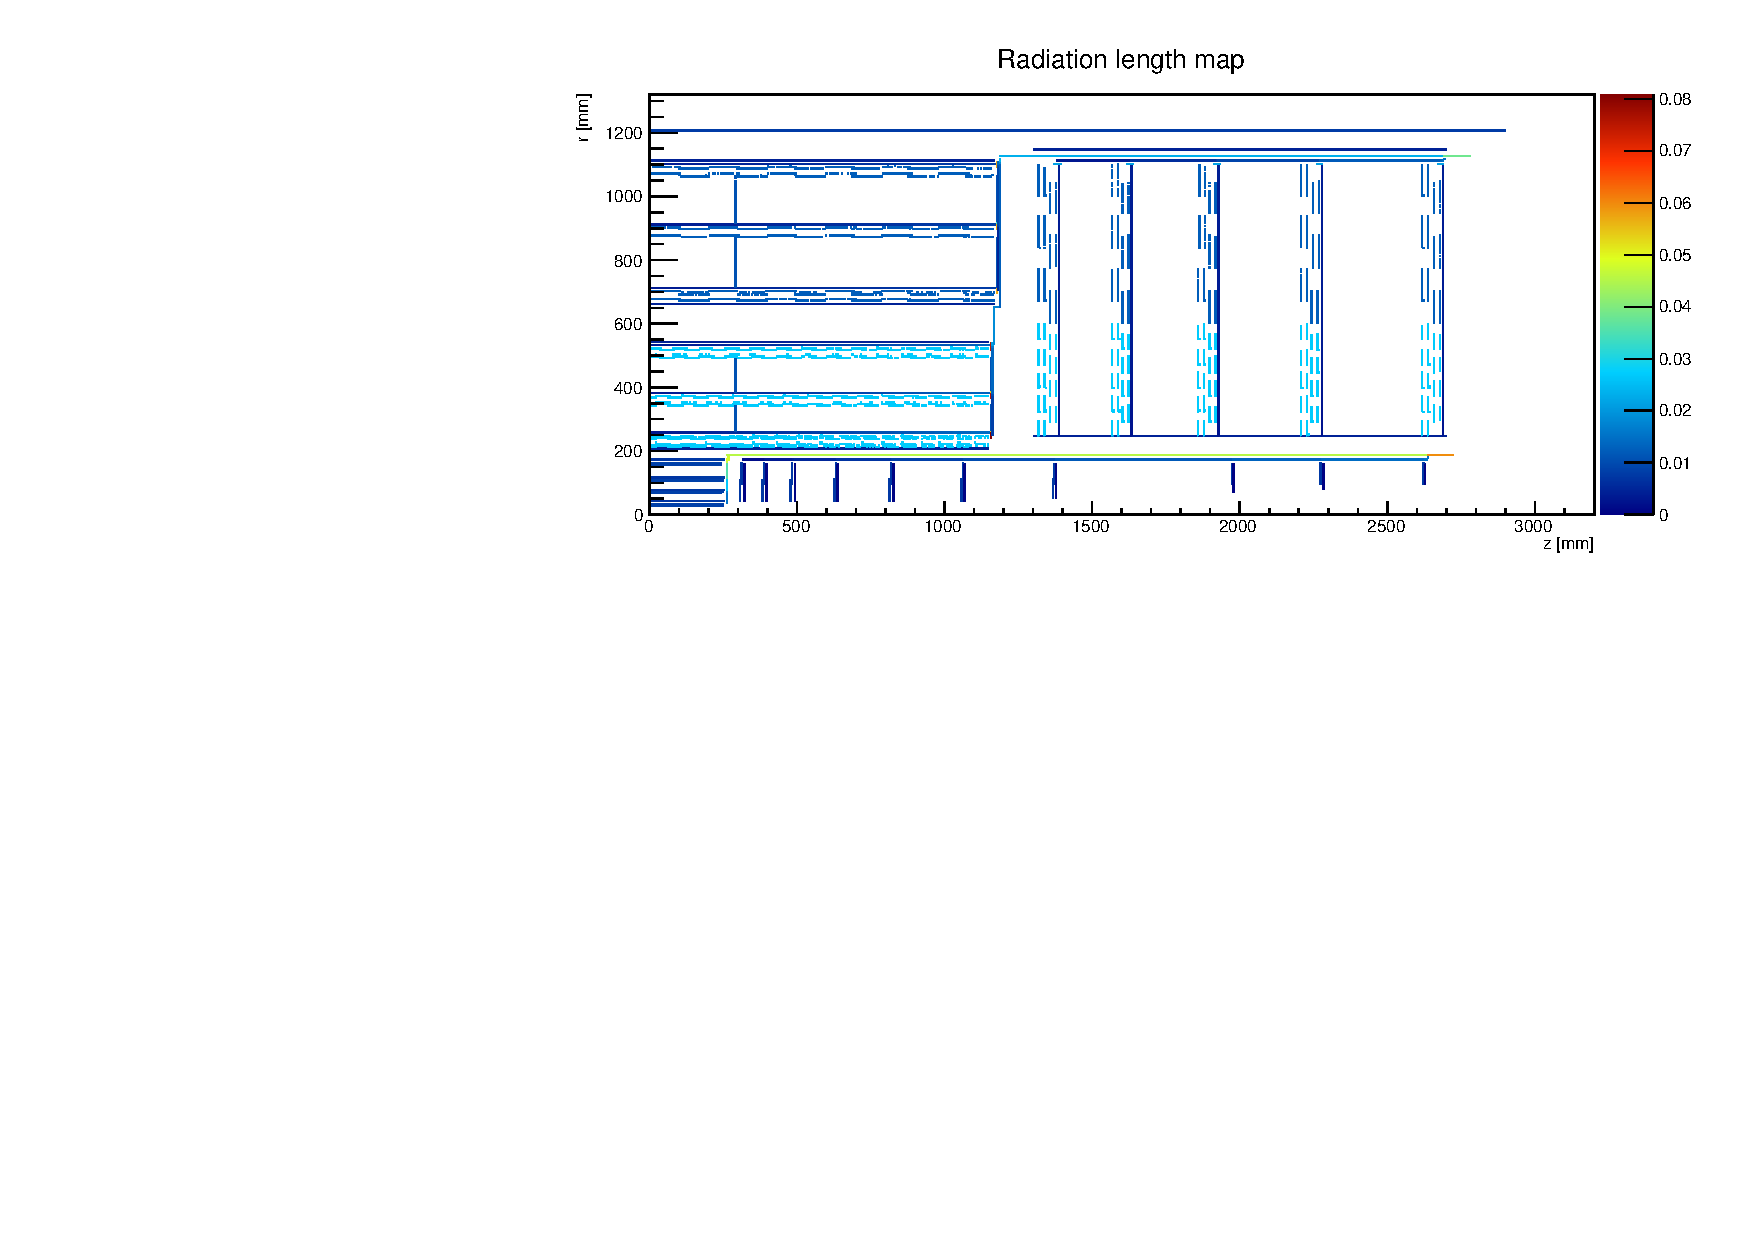
\includegraphics[width=\textwidth]{img/newModel.pdf}
  \end{center}
  \begin{itemize}
    \vspace*{-0.6cm}
  \item Cables material in \alert{dedicated} volumes
    \pause
  \item More \alert{detailed}
    \pause
  \item Better routing \alert{algorithm}
    \begin{itemize}
    \item \alert{automatically} decide where cables go
    \item avoid \alert{collisions}
    \end{itemize}
    \pause
  \item More \alert{functionality}
  \end{itemize}
\end{frame}

\begin{frame}{Advantages}
  \begin{block}{Correct description for \alert{tilted} modules}
    \begin{itemize}
    \item In old model the cables were distributed \alert{inside} the modules
      \begin{itemize}
      \item \alert{wrong} result in case of tilted modules
      \end{itemize}
      \pause
    \item Now is \alert{possible} to model this design
    \end{itemize}
  \end{block}
  \begin{center}
    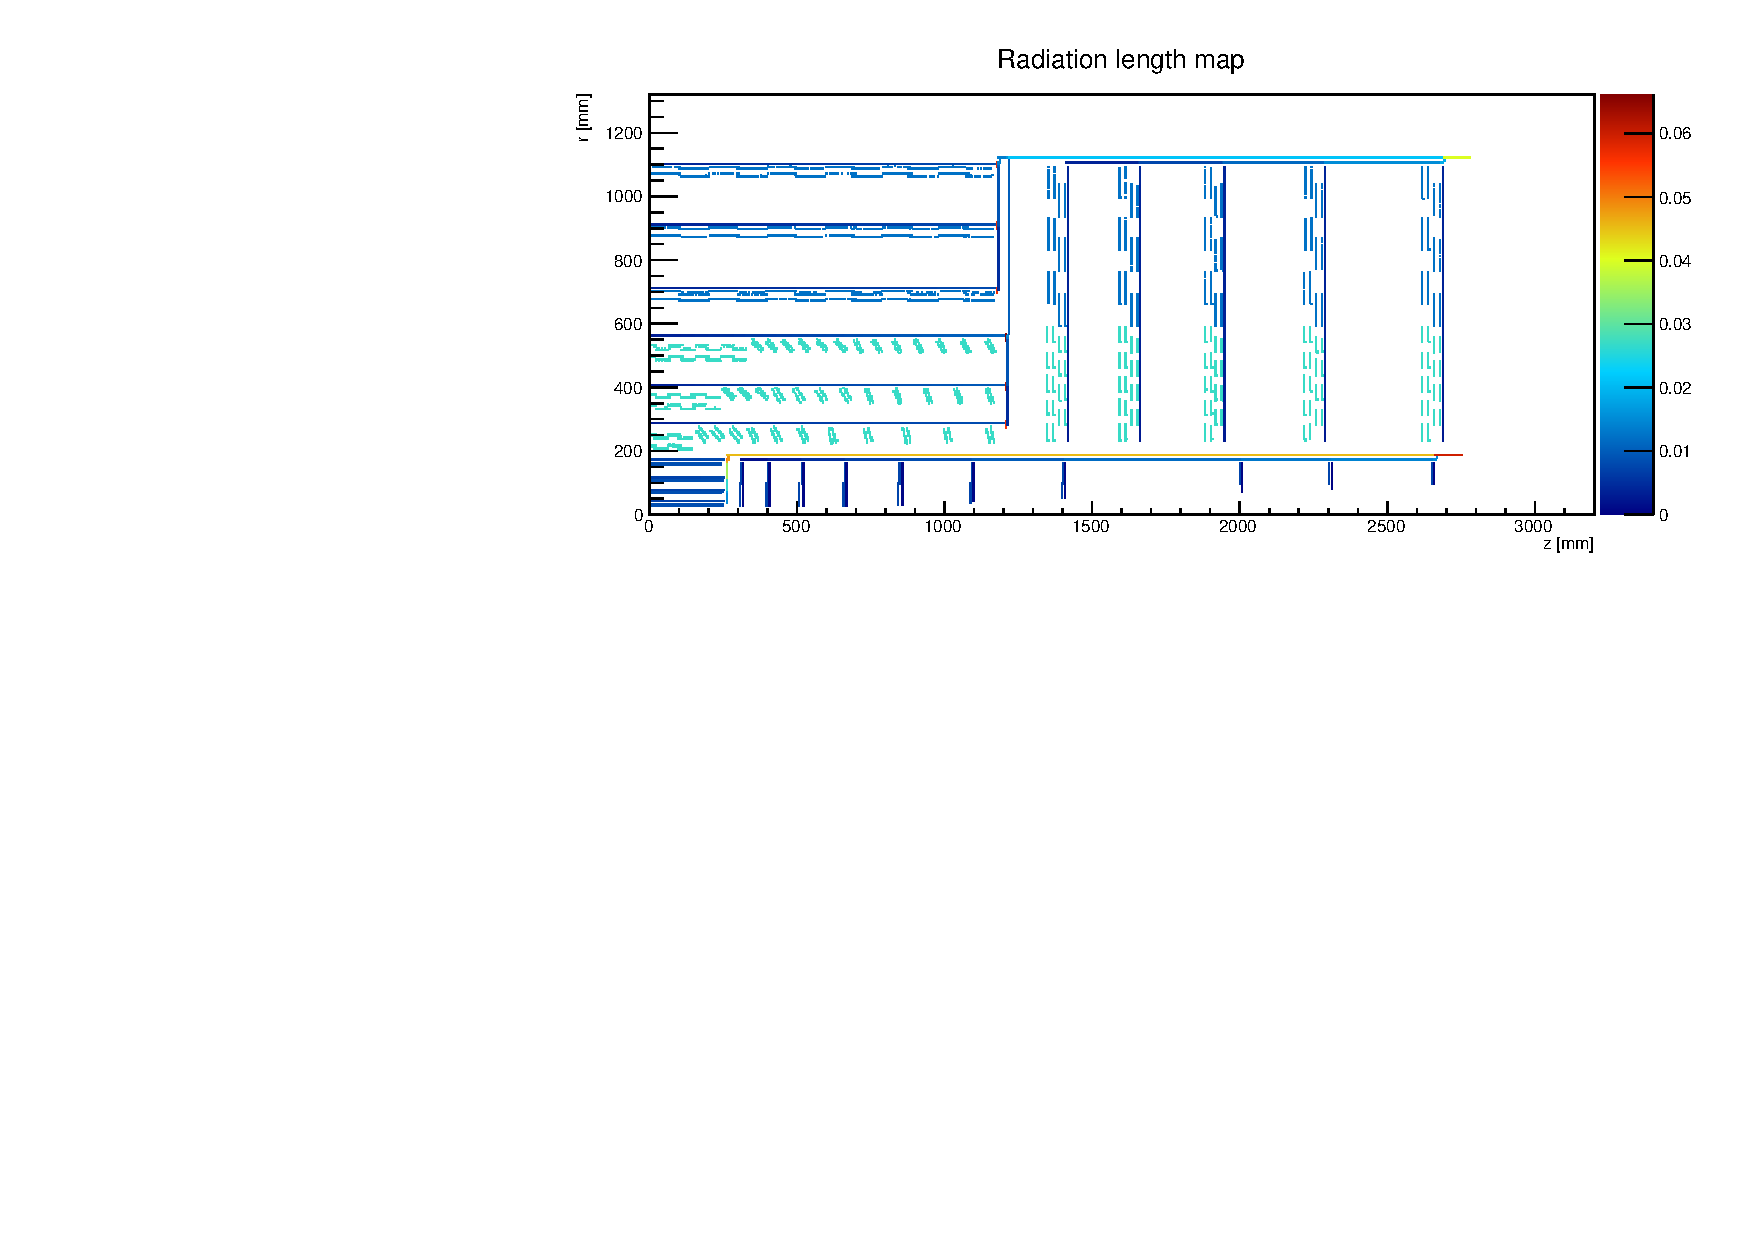
\includegraphics[width=\textwidth]{img/tilted.pdf}
  \end{center}
\end{frame}

\begin{frame}{New feature}
  \begin{block}{Model for \alert{pixel-like} materials}
    \begin{itemize}
    \item All the situations where material \alert{conversion} are \alert{far} from the modules
      \pause
    \item For instance \alert{twisted pair} from modules, electrical optical \alert{transducer}, and \alert{optic fibres} after it
    \end{itemize}
  \end{block}
  \begin{center}
    \only<1>{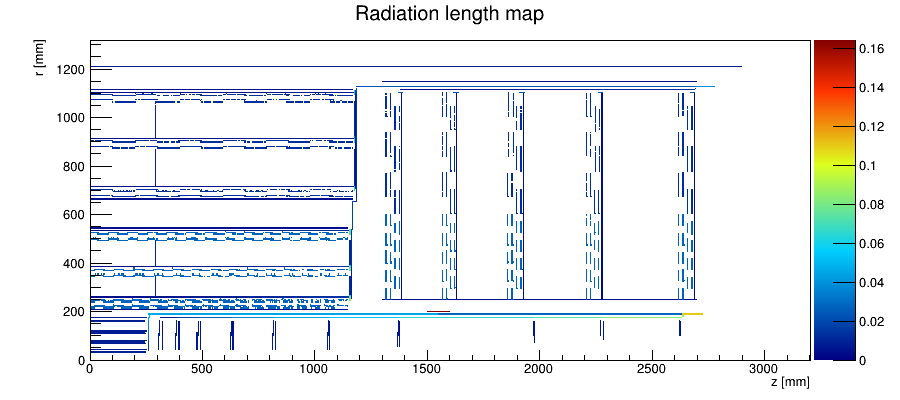
\includegraphics[width=\textwidth]{img/electro-opto.png}}
    \only<2>{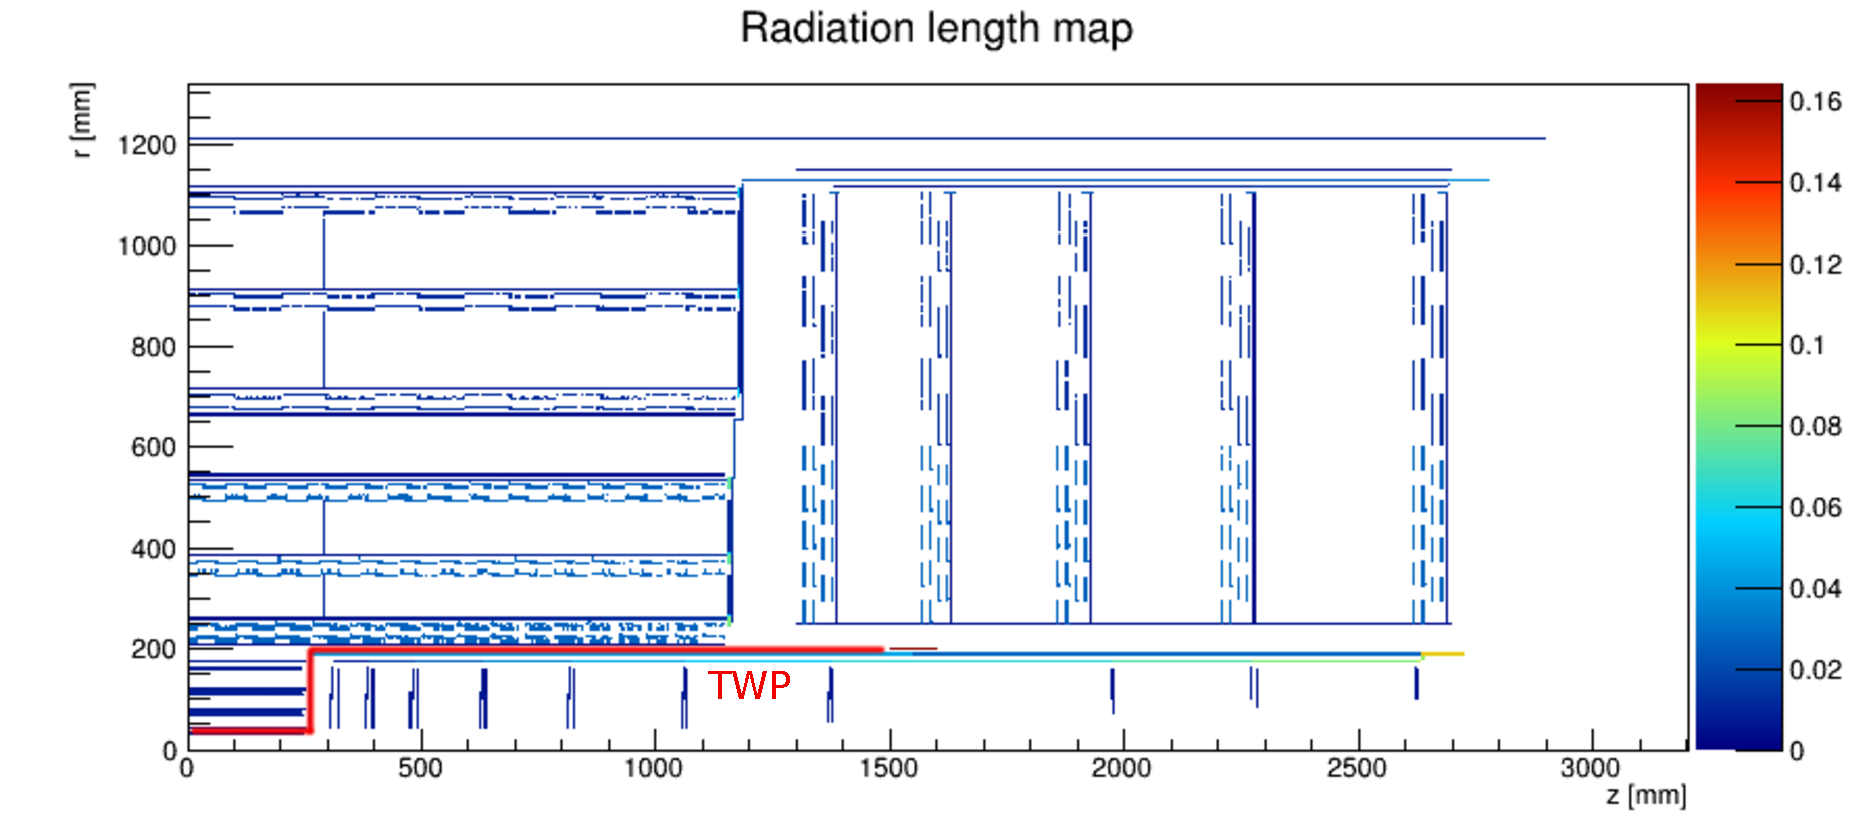
\includegraphics[width=\textwidth]{img/electro-opto1.pdf}}
    \only<3>{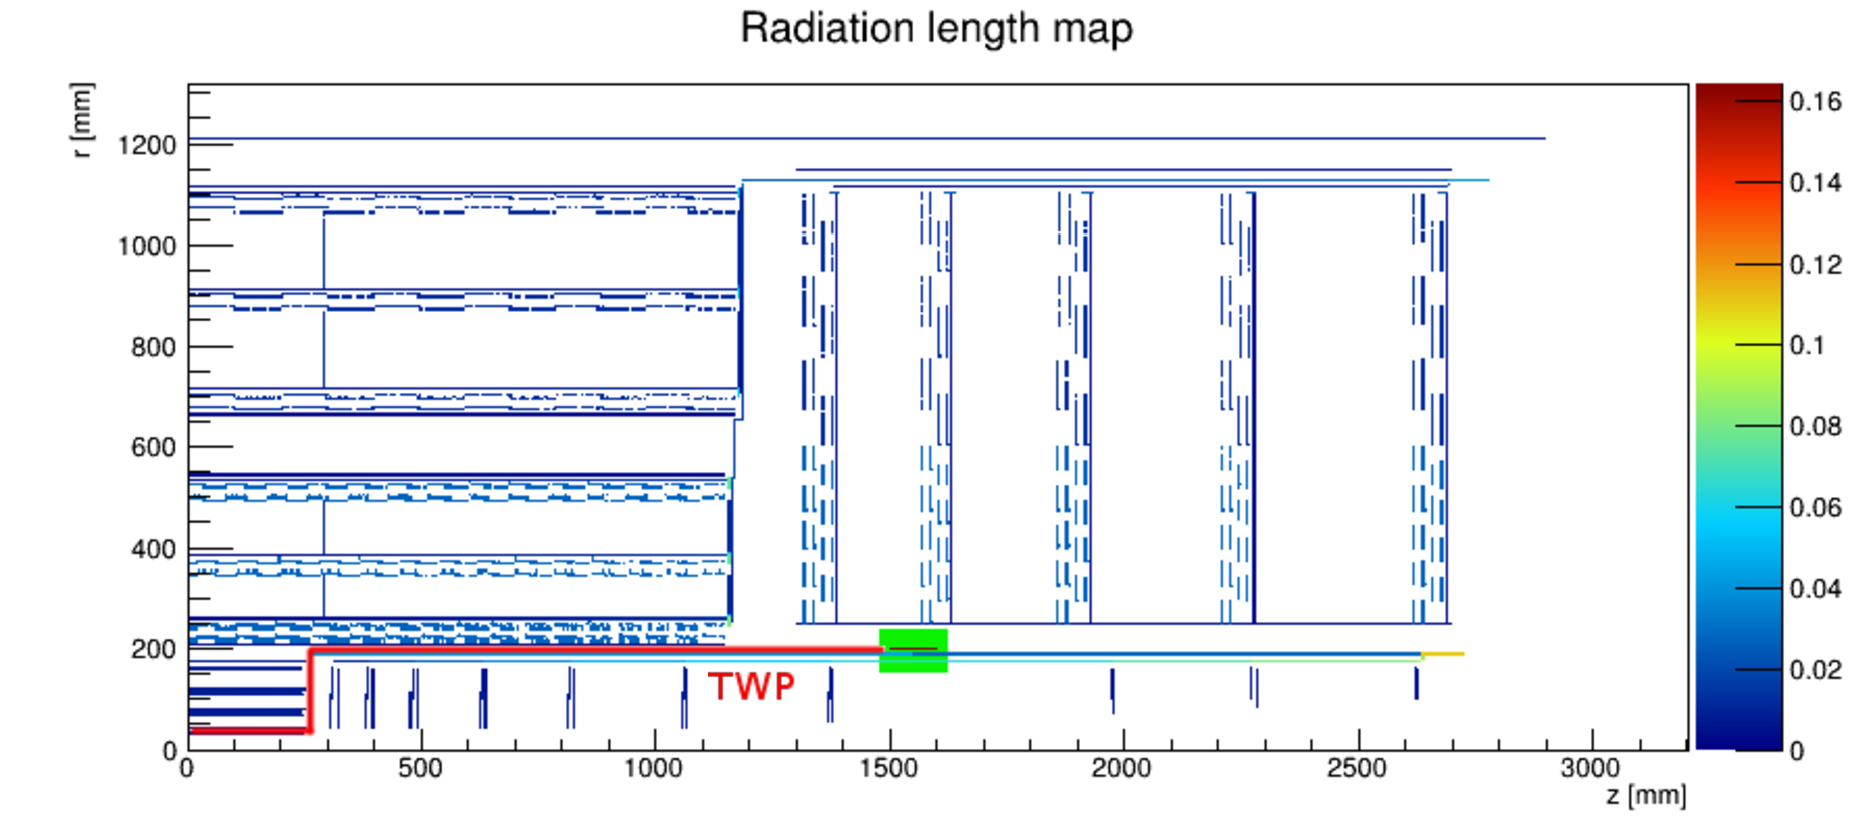
\includegraphics[width=\textwidth]{img/electro-opto2.pdf}}
    \only<4>{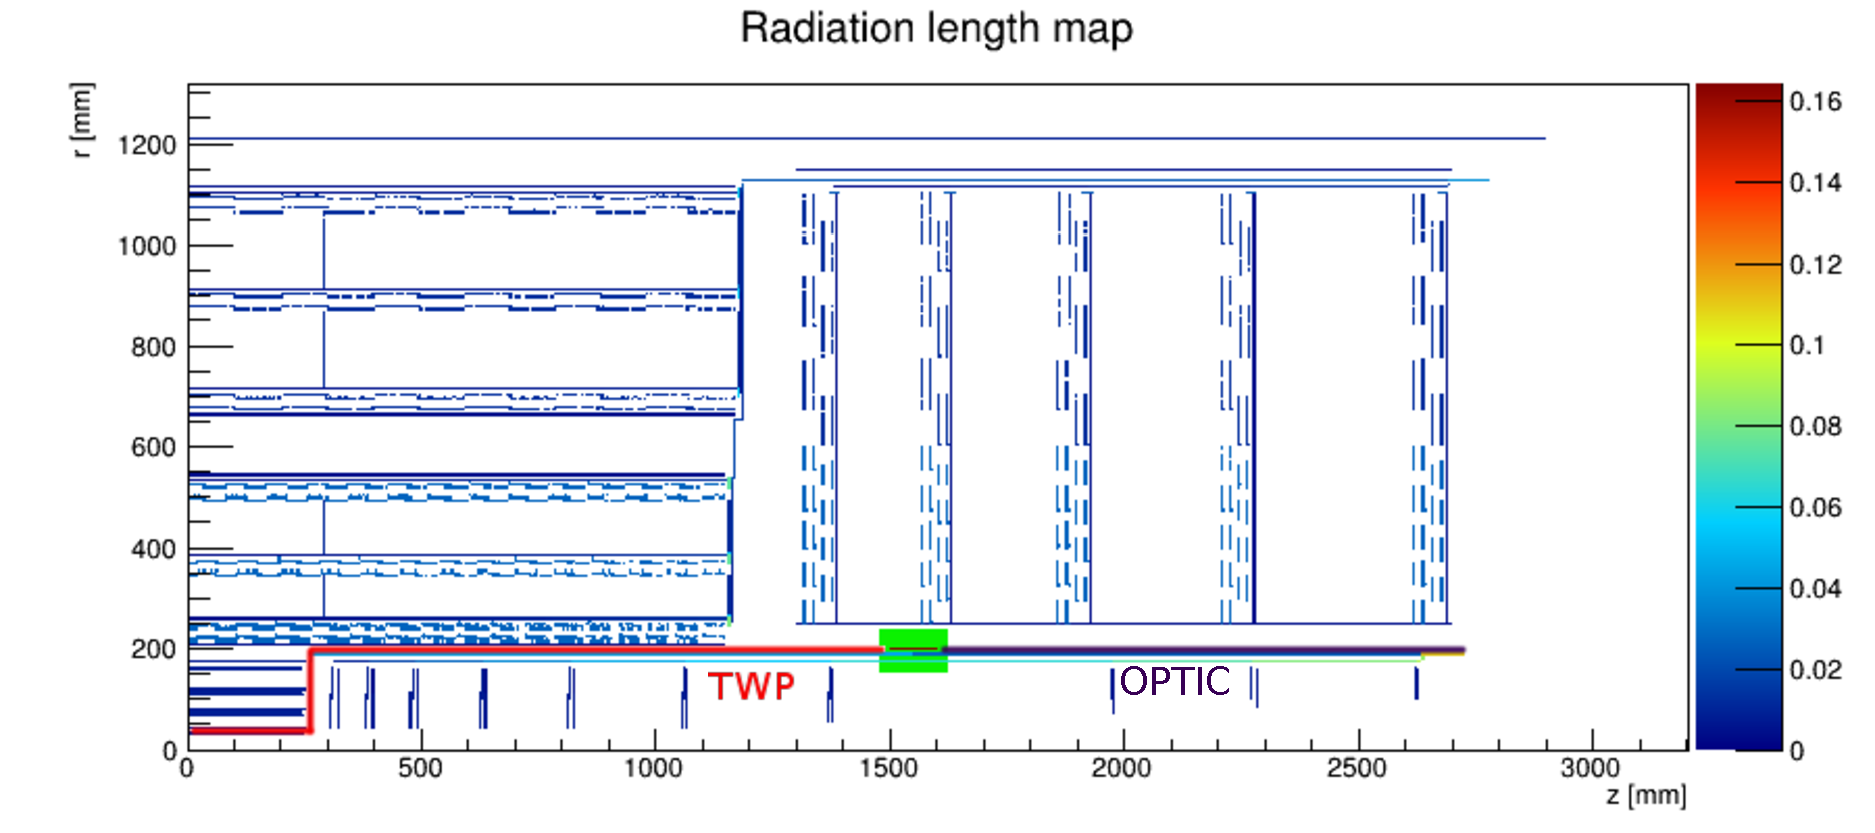
\includegraphics[width=\textwidth]{img/electro-opto3.pdf}}
  \end{center}
\end{frame}

\begin{frame}{Advantages}
  \begin{itemize}
  \item The new algorithm use the \alert{same} underlying c++ objects of the old
    \pause
  \item This means that the \alert{export} to \alert{CMSSW} is working as usual
    \begin{itemize}
    \item only more \alert{detailed} than before
    \end{itemize}
  \end{itemize}
\end{frame}

\begin{frame}{Validation}
  \begin{enumerate}
  \item \alert{Comparison} between old and new models
    \pause
  \item Accurate \alert{tests} new model only with controlled amount of material and exact computation of material amount
  \end{enumerate}
\end{frame}

\begin{frame}
  \begin{block}{Test15 $\rightarrow$ \alert{tested in all possible inputs}}
    \alert{$100 g/m$} of \emph{Cu} in the disk of endcap
    \begin{itemize}
    \item \alert{service} true
    \end{itemize}
  \end{block}
  \begin{center}
    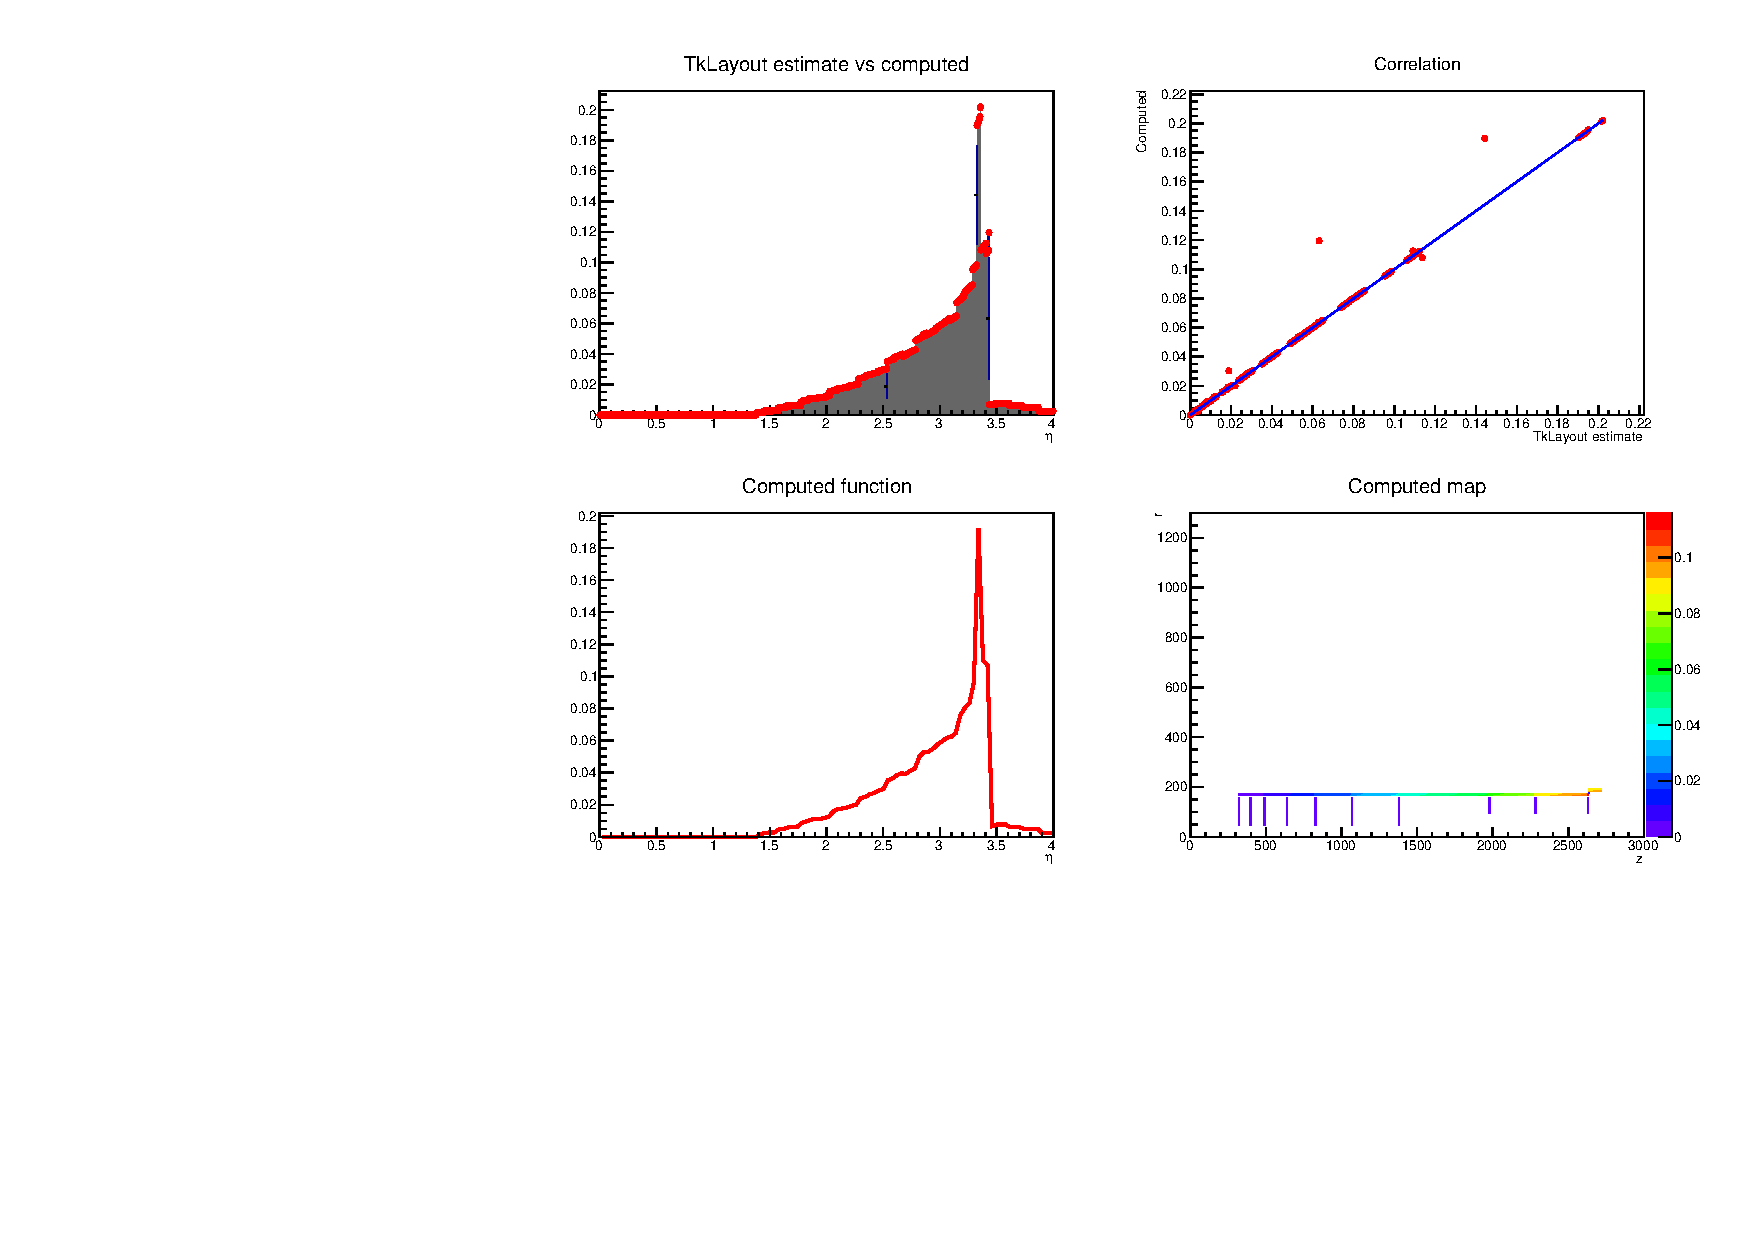
\includegraphics[width=9cm]{img/test15.pdf}
  \end{center}
\end{frame}

\begin{frame}
  \frametitle{Material destination, with different \alert{unit} (g, g/m, mm)}
  \begin{center}
    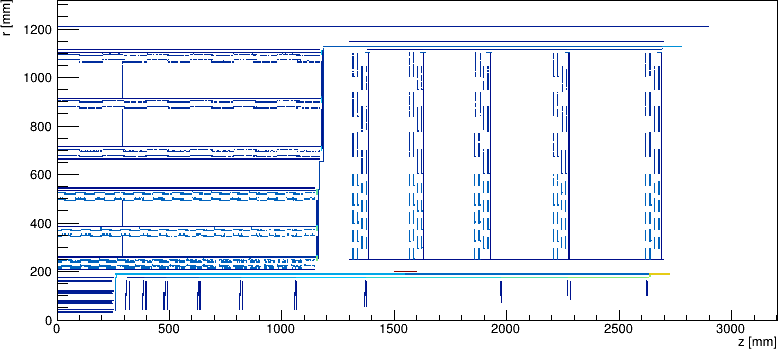
\includegraphics[width=0.85\textwidth]{img/materialScheme.png}
  \end{center}
  \vspace*{-0.8cm}
  \begin{columns}[t]
    \begin{column}{0.47\textwidth}
      \begin{block}{Destination}
        \begin{itemize}
        \item In \alert{module}
          \pause
        \item In \alert{rods}, a series of modules of barrel with same $\phi$
          \pause
        \item In \alert{layers/disks}
        \end{itemize}
      \end{block}
    \end{column}
    \pause
    \begin{column}{0.47\textwidth}
      \begin{block}{Behavior}
        \begin{itemize}
        \item \alert{Locally} (also volumes inside module)
          \pause
        \item as a \alert{service}
          \pause
          \begin{itemize}
          \item can be \alert{converted} in flange or custom position
          \end{itemize}
        \end{itemize}
      \end{block}
    \end{column}
  \end{columns}
\end{frame}


\begin{frame}
  \fontsize{4.5pt}{6pt}\selectfont
  \begin{center}
    \begin{tabular}{|c|c|c|c|}
      \cline{2-4}
      \multicolumn{1}{c|}{} & \color{darkgreen}Unit=$g/m$ & \color{darkgreen}Unit=$mm$ & \color{darkgreen}Unit=$g$\\
      \hline
      \rowhead{\module}{\serfal} & \cont{\module}{$\times \modlen$}{\noacc}{\noconv}{\sca}& \cont{\module}{$\times \modsur\times \rho$ (sensor surface)}{\noacc}{\noconv}{\sca}& \cont{\module}{$\times 1$}{\noacc}{\noconv}{\sca}\\
      \hline
      \rowheadb{\module}{ring $R$ of $N$}{\sertru} & \cont{\follsup}{$\times \nummod_R \times \suplen_i$}{\acc}{\conv (1:1 by default, with warning)}{\sca} & \deprecont{\follsup}{$\times \nummod_R \times \supsur_i \times \rho$}{\acc}{\conv  (1:1 by default, with warning)}{\sca} & \err \\
      \hline
      \rowhead{\rod (barrel)}{\serfal} & \cont{\allsup}{$\times \nummod_1 \times \suplen_i$}{\noacc}{\noconv}{\nosca} & \cont{\allsup}{$\times \supsur_i \times \rho$}{\noacc}{\noconv}{\nosca} & \cont{\allsup}{$\times \nummod_1 \times \frac{\suplen_i}{\sum_{j=1}^N\suplen_j}$}{\noacc}{\noconv}{\nosca} \\
      \hline
      \rowhead{\rod (barrel)}{\sertru} & \cont{\allsup}{$\times \nummod_1 \times \suplen_i$}{\noacc}{\conv}{\nosca} & \deprecont{\allsup}{$\times \supsur_i \times \rho$}{\noacc}{\conv}{\nosca} & \err \\
      \hline
      \rowhead{\layer}{\serfal} & \cont{\allsup}{$\times \suplen_i$}{\noacc}{\noconv}{\nosca} & \cont{\allsup}{$\times \supsur_i \times \rho$}{\noacc}{\noconv}{\nosca} & \cont{\allsup}{$\times \frac{\suplen_i}{\sum_{j=1}^N\suplen_j}$}{\noacc}{\noconv}{\nosca} \\
      \hline
      \rowhead{\layer}{\sertru} & \cont{\allsup}{$\times \suplen_i$}{\noacc}{\conv}{\nosca} & \deprecont{\allsup}{$\times \supsur_i \times \rho$}{\noacc}{\conv}{\nosca} & \err \\
      \hline
    \end{tabular}
  \end{center}
\end{frame}

\begin{frame}[fragile]{Example configuration}
  \tiny
  \begin{columns}[t]
    \begin{column}{0.47\textwidth}
      \begin{block}{\pat{.../Materials/ptPS}}
\begin{verbatim}
Materials module-ptPS {
  type module

  // Default sensor:
  ReferenceSensor 1 {
    numStripsAcross 960
    numSegments 32
  }
  ReferenceSensor 2 {
    numStripsAcross 960
    numSegments 2
  } 

  // Sensor
  Component {
    componentName Sensor
    service false
    scaleOnSensor 0
    targetVolume 1
    Element {
      elementName SenSi
      quantity 0.2
      unit mm
    }
  }
\end{verbatim}
$\cdots$
      \end{block}
    \end{column}
    \begin{column}{0.47\textwidth}
      \begin{block}{\pat{.../Materials/rodPtPS}}
\begin{verbatim}
Materials rodPtPS {
  type rod

  Component {
    componentName Cooling
    service true
    scaleOnSensor 0
    Element {
      elementName Steel
      quantity 7.860696517
      unit g/m
    }
    Element {
      elementName CO2
      quantity 1.791044776
      unit g/m
    }
  }
\end{verbatim}
$\cdots$
      \end{block}
    \end{column}
  \end{columns}
\end{frame}

\begin{frame}[fragile]{Example configuration}
  \tiny
  \begin{columns}[t]
    \begin{column}{0.47\textwidth}
      \begin{block}{\pat{.../Conversions/flange}}
\begin{verbatim}
Station {
  stationName flange
  type flange
...
  Conversion {
    Input {
      Element {
        elementName Cu_MV
        quantity 10
        unit g/m
      }
    }
    Output {
      Element {
        elementName Cu
        quantity 10
        unit g/m
        service true
      }
      Element {
        elementName Cu
        quantity 0.423
        unit g
        service false
      }
\end{verbatim}
$\cdots$
      \end{block}
    \end{column}
    \begin{column}{0.47\textwidth}
      \begin{block}{\pat{.../Conversions/endcap1}}
\begin{verbatim}
Station {
  stationName endcap1
  type second

  minZ 1500
  maxZ 1600

  Conversion {
\end{verbatim}
$\cdots$
      \end{block}
    \end{column}
  \end{columns}
\end{frame}

\begin{frame}
  \begin{block}{Conclusions}
    \begin{itemize}
    \item new material model \alert{finished}
    \item<2-> model validated
    \item<3-> detailed \alert{radiation maps}
    \end{itemize}    
  \end{block}
  \begin{block}<4->{Next steps}
    \begin{itemize}
    \item<4-> develop configuration files for \alert{pixel} and
      \alert{inspect} possibilities
    \item<5-> tracking \& track-trigger performance with \alert{tilted} barrel (within tkLayout) 
    \item<6-> study of \alert{pixel} (vertex resolution \& impact of material on tracking in general)
    \item<7-> \alert{export} of tilted barrel to CMSSW (allows studies in full simulation)
    \end{itemize}
  \end{block}
\end{frame}

\begin{frame}
  $\mathcal{\qquad SO\ \ LONG,}$
  \vspace{0.6cm}

  $\mathcal{\qquad \qquad AND\ \ THANKS\ \ FOR\ \ ALL\ \ THE\ \ FISH.}$
\end{frame}

%BACKUP
\appendix

\section{\appendixname}

\begin{frame}[fragile]
  \frametitle{Outer tracker Bandwidth}
  \begin{center}
    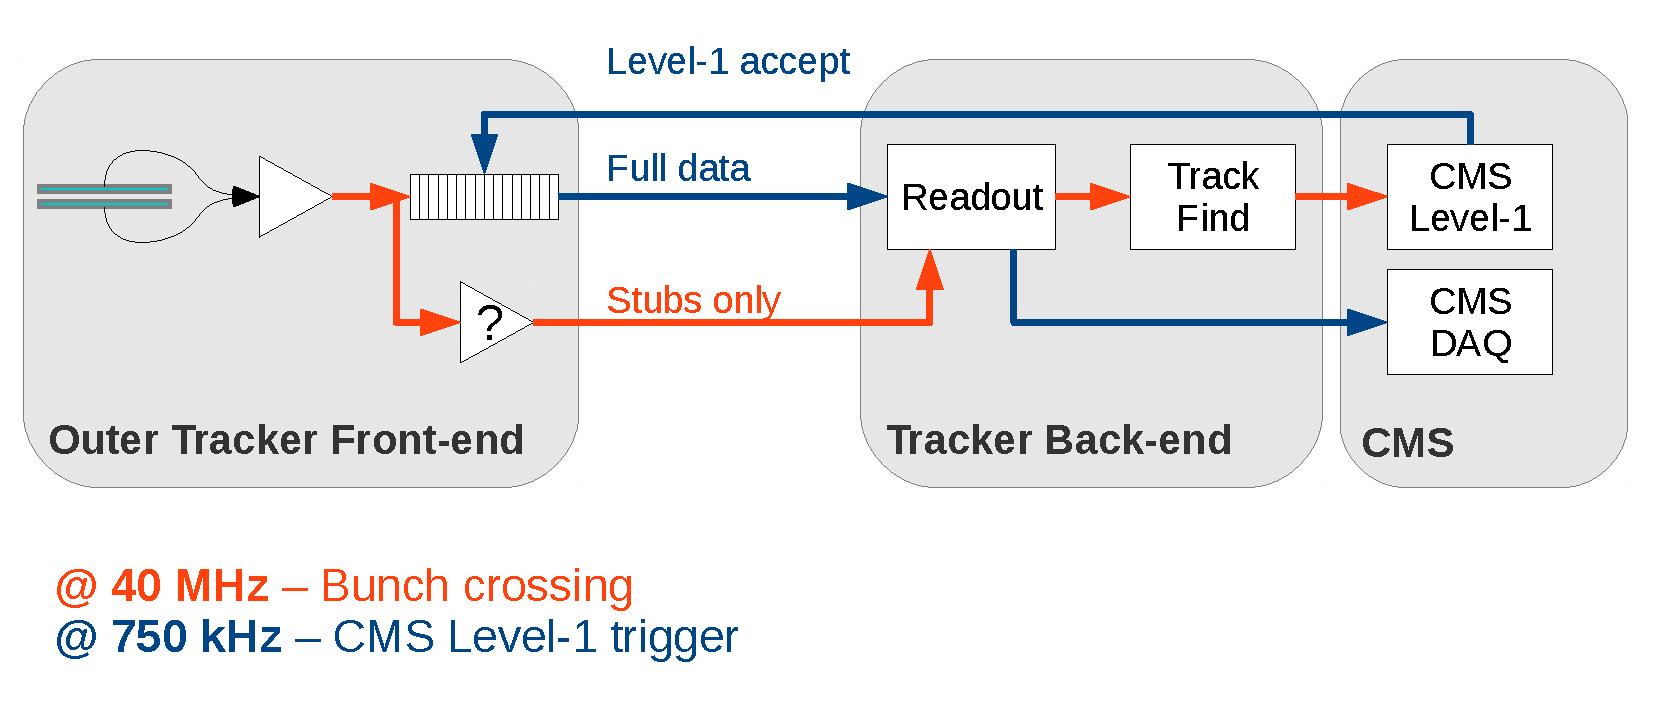
\includegraphics[width=\textwidth]{img/bandwidth.pdf}
  \end{center}
%\tikz[baseline, overlay]\coordinate (band2) at (5cm,3.5cm){};
%\tikz[baseline, overlay]\node<2>[evidenceNode] (band1) at (5cm,0cm){Material for optoelectronics transducers};
%\tikz[baseline, overlay]\path[-latex, bend right, evidenceArrow]<2> (band1) edge (band2);
\end{frame}

\begin{frame}
  \frametitle{Modules}
  \begin{center}
    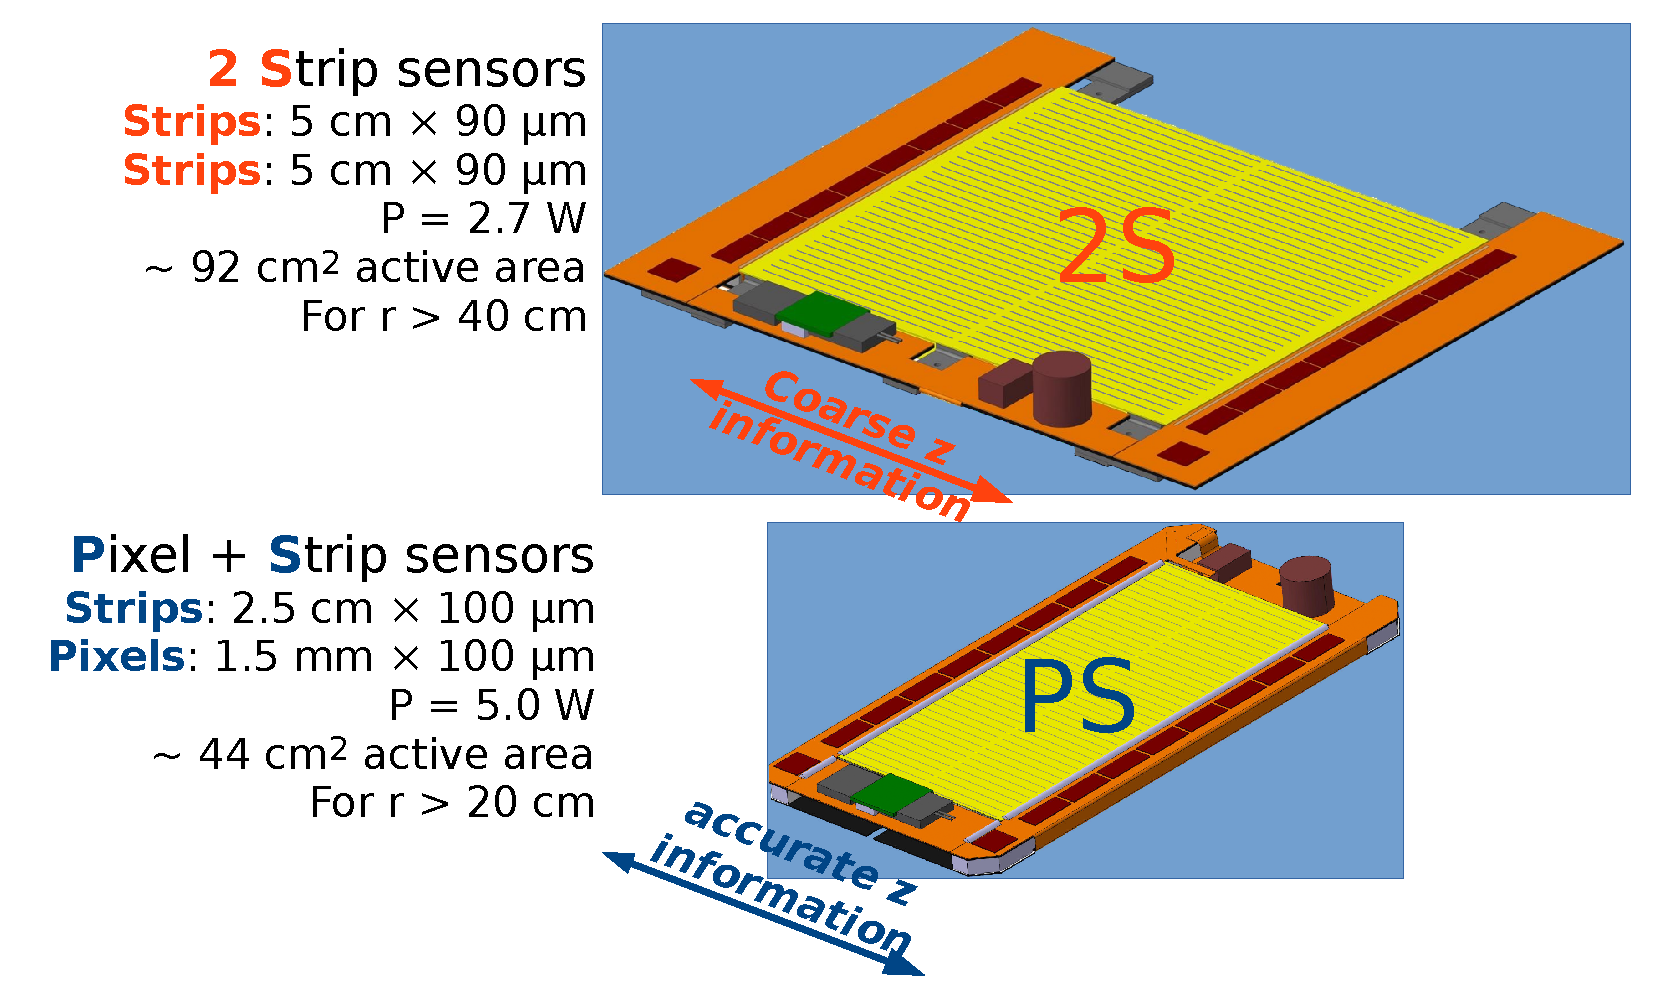
\includegraphics[width=\textwidth]{img/modules.pdf}
  \end{center}
\end{frame}

\begin{frame}
  \frametitle{Pixel Bandwidth}
  \begin{center}
    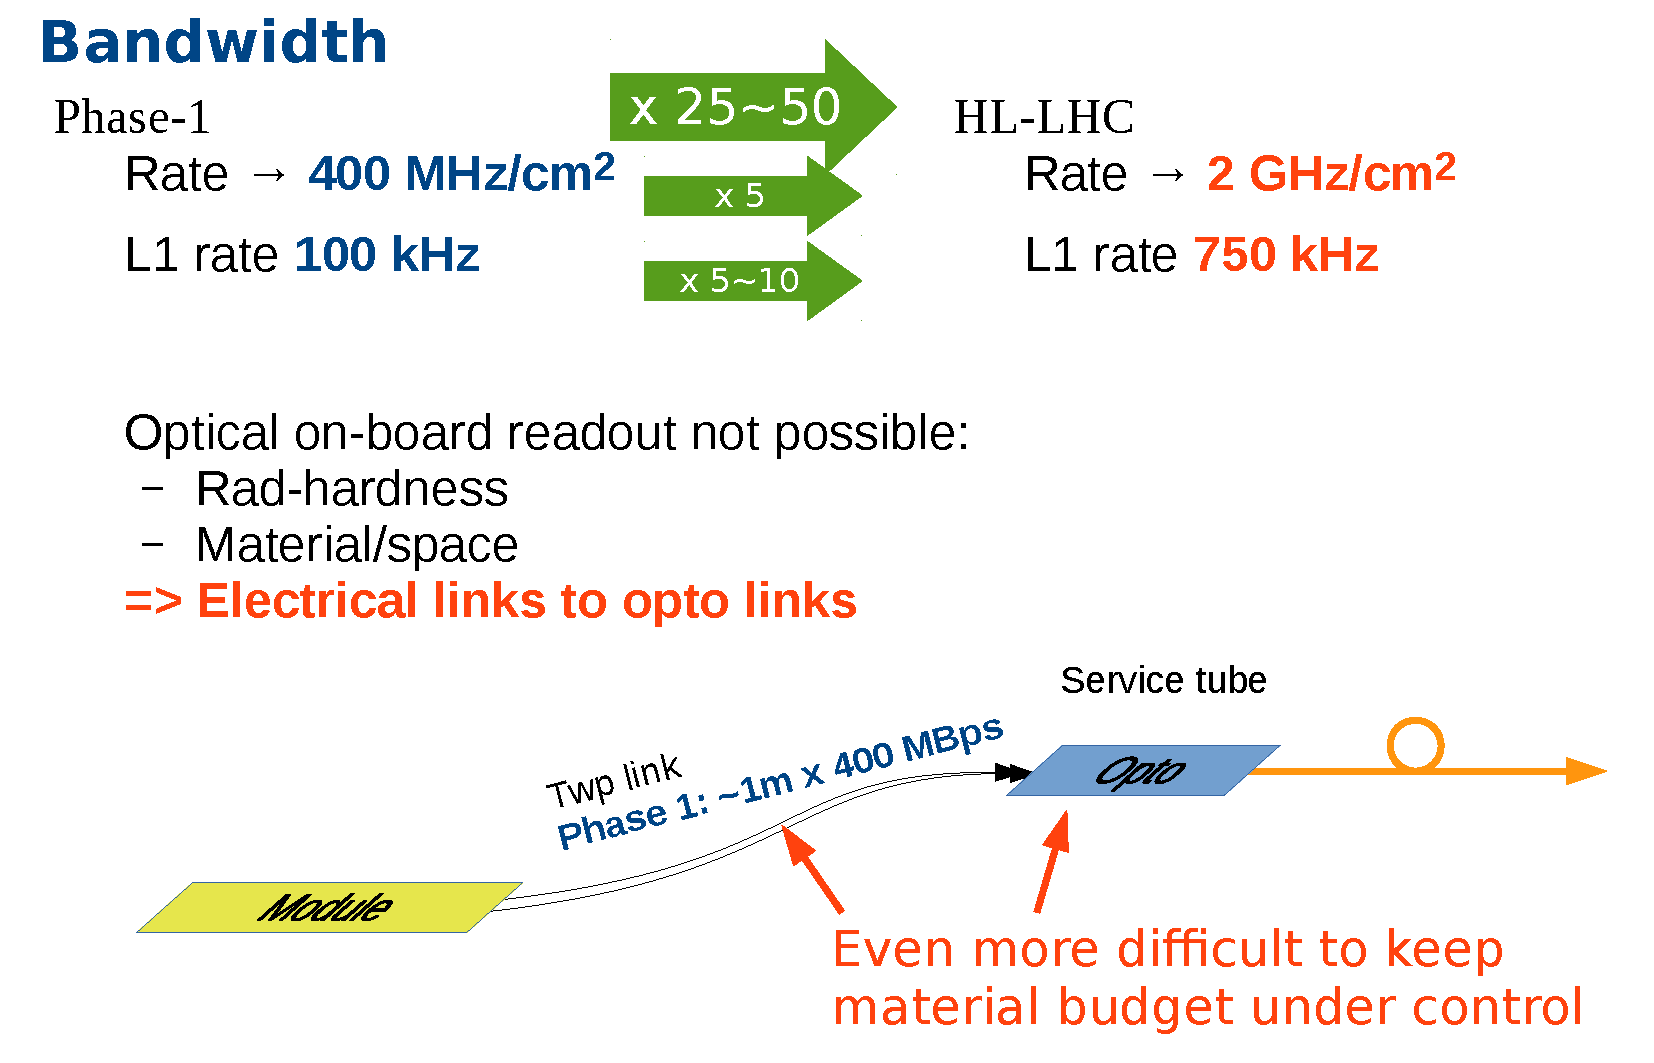
\includegraphics[width=\textwidth]{img/optoele.pdf}
  \end{center}
\end{frame}

\begin{frame}
  \frametitle{Pixel Powering}
  \begin{center}
    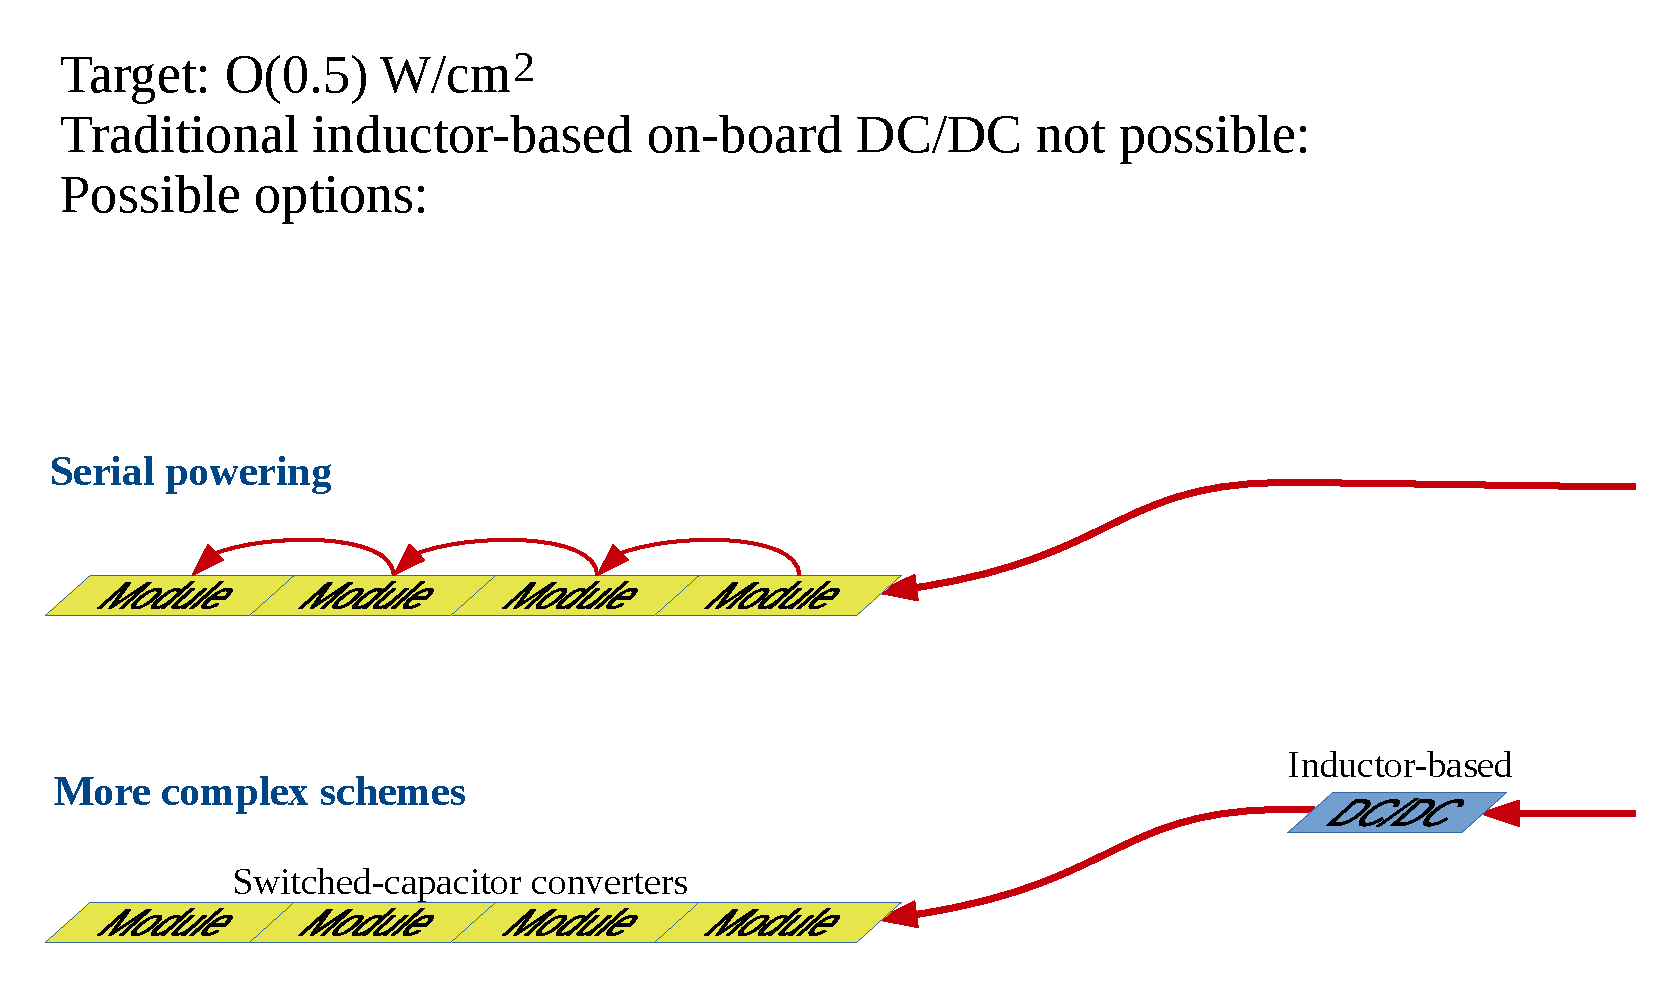
\includegraphics[width=\textwidth]{img/pixelPower.pdf}
  \end{center}
\end{frame}


\end{document}

